\documentclass[11pt]{article}

\usepackage{amsmath,amssymb,amsfonts}
\usepackage{booktabs}
\usepackage{graphicx}
\usepackage{hyperref}
\usepackage[margin=1in]{geometry}
\usepackage[numbers,square,sort&compress]{natbib}
\usepackage{algorithm}
\usepackage{algorithmic}
\usepackage{multirow}
\usepackage{xcolor}
\usepackage{tikz}
\usetikzlibrary{positioning,arrows.meta,shapes.geometric,calc}
\usepackage[affil-it]{authblk}

\renewcommand{\arraystretch}{1.3}

\title{Drug Failures Partition into Two Kinds: Cross-Design Evidence Diagnosis Across Ten Disease Domains}

\author{Elliot Tower}
\affil{Independent researcher \\ \texttt{elliot@elliottower.ai}}

\date{}

\begin{document}
\maketitle

\begin{abstract}
\textbf{Background:}
Mendelian randomization (MR) evidence predicts drug success, but when a drug fails despite genetic support---or succeeds without it---the MR screen alone cannot explain why. We asked whether comparing observational, MR, and RCT evidence can diagnose structurally distinct failure modes.

\textbf{Methods:}
We assembled 41 mechanism families across ten disease domains. Observational and MR effect sizes were standardized to Cohen's $d$ with a fixed $d = 0.10$ threshold. A deterministic rule classified each family by the agreement pattern between observational and MR evidence. A two-stage design separated diagnostic from predictive content by assembling etiologic evidence before examining RCT outcomes.

\textbf{Results:}
MR-only and the cross-design rule produced identical classifications with zero McNemar disagreements across all 32 scored families, because 31 of 32 have non-trivial observational support, making the observational variable near-constant. The pre-registered rule classified 18/22 families correctly (81.8\%, 95\% Wilson CI 61.5--92.7\%, $p < 0.001$). A blind extension added 14 families across seven domains (6/10 correct, 60.0\%, CI 31.3--83.2\%, $p = 0.17$); combined 24/32 ($p = 0.004$). The eight misclassified families partitioned into two structurally distinct groups: three with causal MR (drug failed despite a real mechanism---translation gaps and exposure mismatch) and five with null MR (drug succeeded despite null signal---effector-neutralization and mechanism-bypass). Five named boundary classes offer mechanistic hypotheses for each type of miss.

\textbf{Conclusions:}
The cross-design framework's contribution is diagnostic, not predictive. MR-null status accounts for all predictive power, replicating the genetic-support finding of Nelson et al.\ and Minikel et al. The observational leg adds failure-mode resolution: translation gaps, exposure mismatches, and effector-neutralizations each demand different pipeline responses. Drug failures partition into two kinds---failures of non-mechanisms (null MR) and failures of real mechanisms (causal MR)---a distinction invisible to MR screening alone.
\end{abstract}

\paragraph{Keywords:} Mendelian randomization, drug development, cross-design concordance, evidence triangulation, failure-mode diagnosis, Phase~III trials, drug target validation, pharmacogenomics

\section{Introduction}

Drug development for Alzheimer's disease and multiple sclerosis consumes billions of dollars annually, with an overall AD drug failure rate exceeding 99\% \cite{cummings2014}. Standard tools for evaluating mechanistic evidence---GRADE for rating certainty, $I^2$ for measuring heterogeneity---operate within a single study design. They assess whether twelve RCTs agree, leaving cross-design consistency untested: whether RCT evidence agrees with genetic evidence, or whether observational signals survive Mendelian randomization.

Several independent findings establish that genetic evidence carries information about drug success. \citet{nelson2015} found that drugs with genetic support for their target are twice as likely to reach approval, a finding refined by \citet{minikel2024} with larger datasets. \citet{gill2021} showed that MR concordance with RCTs predicts drug approval. \citet{ference2019} demonstrated that MR-derived causal estimates for cardiovascular targets match RCT efficacy. Triangulation \cite{lawlor2016,munafo2018} captures the intuition that multiple evidence types with independent biases should converge on a true effect. \citet{hammerton2021} formalized the requirement that evidence streams must have unrelated sources of bias for triangulation to strengthen causal inference. The framework provides no standard quantitative test and does not distinguish \emph{types} of convergence failure.

A parallel development in causal inference addresses observational-RCT disagreements directly. \citet{hernan2016} proposed that observational studies should emulate a hypothetical target trial---specifying eligibility, treatment strategies, time zero, and causal contrasts---to minimize biases such as immortal time bias and prevalent-user selection. This resolved the HRT-cardiovascular discrepancy: the Nurses' Health Study's protective signal was an artifact of prevalent-user bias, reconciled with the WHI trial's harmful result via target trial emulation \cite{hernan2008}. Many apparent cross-design discrepancies reflect methodological artifacts rather than biological signals.

Our claim requires precision. We do not argue that observational-RCT disagreement \emph{per se} is informative---the target trial literature shows it often is not. We argue that the pattern across three evidence types (observational, MR, RCT) at the \emph{mechanism-family} level diagnoses failure modes that no single type can identify. MR provides an evidence stream whose biases (pleiotropy, weak instruments, population stratification; \cite{daveysmith2014,gill2024pitfalls}) are largely independent of observational biases (confounding, selection, reverse causation), satisfying the triangulation independence condition \cite{hammerton2021}.

We operationalized this with an explicit decision rule and tested it across three disease domains. An ablation shows that MR evidence alone accounts for all predictive power---the observational leg adds zero classifications beyond what MR provides. The structural explanation: nearly every mechanism family reaching Phase~III has non-trivial observational support (31/32 scored families), so the observational variable is near-constant and carries no discriminative information.

The contribution is diagnostic rather than predictive. A two-stage analysis---first etiologic evidence only, then adding RCT outcomes---reveals three failure modes that MR alone cannot separate: zombie mechanisms, translation gaps, and exposure mismatches. All produce failed drugs; what differs is \emph{why}.

\paragraph{Contributions.}
\begin{itemize}
\item \textbf{Invariance result (\S\ref{sec:ablation}).} MR-only and the cross-design rule produce identical classifications with zero McNemar disagreements across all 32 scored families. This holds at every threshold tested ($d = 0.05$ to $0.20$). The observational leg carries no predictive information; its value is diagnostic.
\item \textbf{Two-way failure partition (\S\ref{sec:two_modes}).} The eight misclassified families split by MR $d$ into two structurally distinct kinds: failures of non-mechanisms (null MR---the target was never causal) and failures of real mechanisms (causal MR---the target is real, the drug is insufficient or misaligned). This partition is data-driven, not imposed.
\item \textbf{Failure-mode taxonomy (\S\ref{sec:two_modes}).} Within the two-way split, a three-way diagnostic taxonomy emerges from the two-stage analysis: zombie mechanisms, translation gaps, and exposure mismatches. Each demands a different pipeline response. Five finer-grained boundary classes are proposed as mechanistic hypotheses on $n = 8$ misses (Table~\ref{tab:provenance}).
\item \textbf{Amyloid dissection (\S\ref{sec:amyloid}).} Etiologic concordance for amyloid is robust; interventional discordance reveals a translation gap invisible to etiologic or MR evidence alone.
\item \textbf{Robustness (\S\ref{sec:robustness}).} Threshold sensitivity, leave-one-domain-out cross-validation, alternative granularity schemes, and instrument independence audit confirm the result is not driven by threshold choice, any single domain, or family-definition decisions.
\end{itemize}

\section{Materials and Methods}

\subsection{Data}

We assembled 76 neuroepidemiology claims across 24 mechanism families spanning AD and MS. The analysis was subsequently extended to cardiometabolic, autoimmune, oncology, respiratory, metabolic/endocrine, psychiatry, gastroenterology, ophthalmology, and musculoskeletal domains (\S\ref{sec:cardio}--\S\ref{sec:extension}), bringing the total to 41 mechanism families across ten disease domains. Each claim was coded with its mechanism family, study design (observational, MR, genetic, RCT, diagnostic), effect size estimate, confidence interval, and sample size. Effect sizes on ratio scales were converted to Cohen's $d$ using the \citet{chinn2000} formula:
\begin{equation}
d = \frac{|\ln(\text{OR})| \cdot \sqrt{3}}{\pi}, \qquad
\text{SE}_d = \frac{(\ln\text{CI}_{\text{upper}} - \ln\text{CI}_{\text{lower}})}{2 \times 1.96} \cdot \frac{\sqrt{3}}{\pi}.
\label{eq:chinn}
\end{equation}
Hazard ratios were treated as odds ratios for conversion, an approximation that holds when the outcome is rare; all neuroepidemiology outcomes in this dataset satisfy this condition (AD and MS incidence $< 5\%$ in the study populations). For example, Anti-CD20-MS has MR OR = 0.83, yielding $d = |\ln(0.83)| \times \sqrt{3}/\pi = 0.103$. Sources were published systematic reviews, meta-analyses, MR studies, and landmark RCTs. A machine-readable table of all 41 families with effect sizes, confidence intervals, gene targets, instrument types, and classifications is provided as Supplementary Table~S1.

We supplemented the original catalog with etiologic evidence for three families identified through systematic literature search:

\textbf{Anti-CD20-MS.} MR evidence shows that per-SD higher circulating FCRL3 protein is protective against MS (OR~0.83, 95\% CI 0.79--0.89; \cite{lin2023}). Observational B-cell depletion efficacy data from \citet{hu2019}. A CD40 genetic association (OR~1.16; \cite{sokolova2013}) provides corroborating GWAS evidence.

\textbf{HRT-AD.} Observational meta-analysis (protective, OR~0.67, 95\% CI 0.58--0.78; \cite{song2020}) and MR for estradiol (null, OR~1.00, 95\% CI 0.85--1.18; \cite{barth2025}). An ESR1 genetic association (OR~1.14; \cite{cheng2014}) provides corroborating GWAS evidence.

\textbf{Vitamin~D-MS (supplemented).} Observational cohort evidence for low vitamin~D and MS risk (OR~1.40, 95\% CI 1.19--1.64; \cite{munger2006}), added to the existing MR entry.

\subsection{Evidence classification: etiologic versus interventional}

We divided evidence types into two categories. \emph{Etiologic evidence} captures the observational and genetic case for a mechanism: cohort and case-control studies, Mendelian randomization, GWAS, and diagnostic accuracy studies. These ask ``is this mechanism involved in the disease?'' \emph{Interventional evidence} captures the treatment case: randomized controlled trials. These ask ``does intervening on this mechanism help?''

The separation matters because interventional evidence for a mechanism family contains information about the drug outcomes we want to classify. A family's RCT arm is computed from the same trials whose outcomes appear in the holdout. Using it in both places is circular. Etiologic evidence is independent of drug outcomes by construction: neither cohort studies nor MR analyses are causally downstream of whether a drug was approved, so their inclusion in the classification introduces no circularity.

Within etiologic evidence, MR and GWAS studies were pooled into a single ``genetic/causal'' (GEN) evidence type for the concordance rule. This is a pragmatic choice, not an epistemological claim that GWAS susceptibility estimates and MR causal estimates answer the same question---they do not. GWAS estimates disease susceptibility associated with a variant; MR estimates the causal effect of modifying an exposure. The pooling is justified on scale grounds: common variant GWAS effect sizes are inherently small (OR~1.1--1.3 for genome-wide significant hits) even for real causal pathways, and treating them as a separate evidence type would systematically misclassify real GWAS signals as ``null'' against the $d = 0.10$ threshold. The two evidence types in the classification are therefore OBS (observational and diagnostic studies) and GEN (MR and genetic association studies).

\subsection{Cross-design concordance rule}

For each mechanism family, the classification uses two standardized effect sizes: one from observational evidence (OBS) and one from MR/genetic evidence (GEN). When multiple studies exist within a type, we select the most representative published estimate (typically from the largest meta-analysis or most recent MR study). Effect sizes on ratio scales are converted to Cohen's $d$ via Equation~\ref{eq:chinn}. For autoimmune families where case-control standardized mean differences (SMDs) are the natural OBS measure, SMDs enter directly without Chinn conversion.

Each evidence type is classified independently using a two-criterion rule:

\textbf{OBS classification.} Non-trivial if $d_{\text{OBS}} \geq 0.10$; trivial otherwise. The threshold follows Cohen's boundary for negligible effects and is fixed a priori.

\textbf{MR classification.} Causal if (a) the confidence interval excludes the null \emph{and} (b) $d_{\text{MR}} \geq 0.10$; null otherwise. Both criteria must be met---a statistically significant but negligible effect and a large but imprecise effect are both classified as null.

The family-level classification follows from the combination:

\textbf{Qualitative discordance.} OBS non-trivial, MR null. The observational signal does not survive causal testing; the apparent association reflects confounding or reverse causation.

\textbf{Concordance.} OBS non-trivial, MR causal. Both evidence types support the mechanism.

\textbf{Null concordance.} OBS trivial, MR null. No evidence from either type; prediction is ambiguous.

\textbf{Genetic-only signal.} OBS trivial, MR causal. Genetic support without observational confirmation.

This rule operationalizes triangulation \cite{lawlor2016} with an explicit, deterministic decision procedure. Unlike Cochran's $Q$, which assumes all estimates target the same parameter, the concordance rule treats observational and MR estimates as addressing different questions (``is this mechanism associated with disease?'' vs.\ ``is this mechanism causal for disease?'') and classifies their \emph{agreement pattern} rather than testing whether their magnitudes are statistically distinguishable.

\subsection{MR effect-size scaling}

MR effect sizes enter the classification on their native contrast (per-SD, per-unit, or per-genotype). The Chinn $d$ inherits whatever comparison the OR encodes. One family (IL-6R) reports a per-allele OR; this is rescaled to per-SD before Chinn conversion using $\text{OR}_{\text{per-SD}} = \text{OR}_{\text{per-allele}}^{1/\sigma}$ where $\sigma$ is the SD of the exposure per allele. All other MR ORs enter without rescaling. The $d = 0.10$ threshold is applied uniformly across contrasts as a pragmatic choice; we identify threshold-sensitive families in the sensitivity analysis (\S\ref{sec:limitations}).

\subsection{Unit of analysis}

The unit of analysis is the mechanism family, not the individual drug or the target-indication pair. A mechanism family groups drugs that act on the same biological pathway (e.g., ``Anti-CD20-MS'' includes ocrelizumab, rituximab, ofatumumab, and ublituximab; ``Amyloid-AD'' includes BACE inhibitors and immunotherapies targeting amyloid clearance). This granularity matches the MR instrument: a cis-pQTL for FCRL3 indexes B-cell biology, not the pharmacokinetics of any individual antibody. The diagnostic taxonomy classifies pathways, not compounds---a ``zombie mechanism'' means the pathway is non-causal, regardless of which drug targets it. Family definitions are a degree of freedom; we test sensitivity to alternative granularity choices (merging Niacin/HDL into HDL/CETP, splitting Amyloid-AD by sub-mechanism) in the robustness analyses (\S\ref{sec:robustness}).

\subsection{Failure taxonomy}

Three mechanistically defined failure modes follow from the two-stage analysis:

\textbf{Zombie mechanism} (so called because the observational association persists after the causal pathway has been shown to be dead). Etiologic evidence is qualitatively discordant---the MR signal is null while the observational association persists. The observational signal reflects confounding or reverse causation; the mechanism is a statistical association, not a causal pathway. Drugs targeting zombies fail because there is nothing causal to intervene on.

\textbf{Translation-gap mechanism.} Etiologic evidence is concordant (the mechanism is genuinely causal), but drugs targeting it fail or produce marginal benefit. The intervention cannot reverse established downstream pathology at the stage of clinical disease. Etiologic evidence alone classifies these as concordant; only RCT evidence reveals the gap.

A third pattern, \textbf{exposure mismatch}, appears when the MR instrument captures a real causal relationship but the drug targets a different exposure window or delivery route (e.g., lifelong genetic vitamin~D status vs.\ adult oral supplementation).

\subsection{Phase~III holdout}

We assembled 38 Phase~III AD and MS drugs with known outcomes (22 failed, 16 approved). For each drug, we mapped its mechanism to a family classification. Drugs whose family lacked classification received no prediction. The rule was mechanical: qualitative discordance (non-trivial OBS, null MR) classifies as failure; concordance (non-trivial OBS, causal MR) classifies as approval.

\subsection{Two-stage analysis design}

\textbf{Stage~1 (de-circularized).} Classify families using only etiologic evidence. All drug outcomes are fully out of sample. This stage can use ``predicts'' language.

\textbf{Stage~2 (retrospective).} Add interventional evidence and reclassify. Drug outcomes are no longer independent of the classification. This stage uses ``is associated with'' language and examines what the additional evidence reveals.

\subsection{Decision rule}

The complete classification procedure is given in Algorithm~\ref{alg:discordance}. The procedure takes published effect sizes as input and returns a family-level classification with no fitted parameters. Each effect size is converted to Cohen's $d$ (ORs via Chinn; SMDs directly). The OBS and MR legs are classified independently against the $d = 0.10$ threshold, and the family classification follows from their combination. The procedure is deterministic, requires no training data, and can be executed by hand with a calculator.

\begin{algorithm}[t]
\caption{Cross-Design Concordance Classification}
\label{alg:discordance}
\begin{algorithmic}[1]
\REQUIRE Mechanism families $\mathcal{F} = \{f_1, \ldots, f_m\}$; for each $f_j$: effect sizes $d_{\text{OBS}}$, $d_{\text{MR}}$, and MR confidence interval $(l, u)$
\medskip
\STATE \textbf{Standardize.} Convert ORs to $d$ via Eq.~\ref{eq:chinn}; SMDs enter directly
\STATE \textbf{Rescale.} If MR OR is per-allele, rescale to per-SD before conversion
\medskip
\FOR{each family $f_j$}
  \STATE \textbf{OBS:} \textsc{Non-trivial} if $d_{\text{OBS}} \geq 0.10$; else \textsc{Trivial}
  \STATE \textbf{MR:} \textsc{Causal} if $1.0 \notin (l, u)$ \textbf{and} $d_{\text{MR}} \geq 0.10$; else \textsc{Null}
  \IF{\textsc{Non-trivial} and \textsc{Null}}
    \STATE $\text{label}(f_j) \leftarrow$ \textsc{Qualitative Discordance} $\rightarrow$ predict \textsc{Failure}
  \ELSIF{\textsc{Non-trivial} and \textsc{Causal}}
    \STATE $\text{label}(f_j) \leftarrow$ \textsc{Concordance} $\rightarrow$ predict \textsc{Success}
  \ELSIF{\textsc{Trivial} and \textsc{Null}}
    \STATE $\text{label}(f_j) \leftarrow$ \textsc{Null Concordance} $\rightarrow$ \textsc{Ambiguous}
  \ELSIF{\textsc{Trivial} and \textsc{Causal}}
    \STATE $\text{label}(f_j) \leftarrow$ \textsc{Genetic-Only} $\rightarrow$ predict \textsc{Success}
  \ENDIF
\ENDFOR
\medskip
\ENSURE For each drug mapped to family $f_j$: predicted outcome $\in \{\textsc{Success}, \textsc{Failure}, \textsc{Ambiguous}\}$
\end{algorithmic}
\end{algorithm}

\subsection{Ablation design}

To test whether the observational leg contributes predictive power beyond MR alone, we compared four classification rules on all scored families (those with known drug outcomes, excluding pending and construct-limited):

\begin{enumerate}
\item \textbf{Always-fail}: predict failure for every family (base-rate baseline).
\item \textbf{MR-only}: predict failure if MR is null, success if MR is causal (ignore OBS).
\item \textbf{OBS-only}: predict success if OBS is non-trivial, failure if OBS is trivial (ignore MR).
\item \textbf{Cross-design}: the full concordance rule (Algorithm~\ref{alg:discordance}).
\end{enumerate}

For each rule we report total accuracy, accuracy split by outcome (correct failures vs.\ correct approvals), and McNemar paired disagreements between the cross-design and MR-only rules---naming the specific families where the rules diverge, if any.

\begin{figure}[t]
\centering

\includegraphics[width=0.85\textwidth]{figures/fig1_flowchart.pdf}
\caption{\textbf{Classification procedure.}
For each mechanism family, observational and MR effect sizes are
standardized to Cohen's $d$ and classified independently against the
$d = 0.10$ threshold. The family-level classification follows from the
OBS$\times$MR combination: qualitative discordance (non-trivial OBS,
null MR) predicts failure; concordance predicts success.
Stage~1 uses etiologic evidence only; Stage~2 adds RCT outcomes to
diagnose failure modes.}
\label{fig:flowchart}
\end{figure}

\section{Results}

\subsection{Family accounting}
\label{sec:accounting}

Table~\ref{tab:accounting} reconciles all denominators used in this paper. We assembled 27 mechanism families across three disease domains. Five are excluded from the scored set: three with pending trial outcomes (BMI-MS, Lp(a), IL-6R), one construct-limited (IL-4R$\alpha$-AD, where the MR instrument and the drug target different ligands), and one ambiguous (uric acid, where MR estimates depend on the method used). The remaining 22 families have unambiguous drug outcomes and enter the ablation and accuracy analyses.

\begin{table}[t]
\centering
\caption{Family accounting across ten domains. ``Pending'' = no Phase~III readout; ``Constr.'' = construct-limited; ``Ambig.'' = ambiguous MR evidence. The 38-drug holdout (\S\ref{sec:stage1}) is a separate drug-level accounting within neuroepidemiology. Extension domains (\S\ref{sec:extension}) add 14 families across seven disease domains in two blind amendments.}
\label{tab:accounting}
\small
\begin{tabular}{lccccccc}
\toprule
Domain & Total & Pending & Constr. & Ambig. & Scored & Correct & Accuracy \\
\midrule
Neuroepidemiology & 9 & 1 & 0 & 0 & 8 & 7 & 7/8 \\
Cardiometabolic & 10 & 2 & 0 & 1 & 7 & 7 & 7/7 \\
Autoimmune & 8 & 0 & 1 & 0 & 7 & 4 & 4/7 \\
\midrule
\emph{Original total} & \emph{27} & \emph{3} & \emph{1} & \emph{1} & \emph{22} & \emph{18} & \emph{18/22} \\
\midrule
Oncology & 3 & 0 & 0 & 0 & 3 & 1 & 1/3 \\
Respiratory & 3 & 0 & 2 & 0 & 1 & 1 & 1/1 \\
Metabolic/Endocrine & 3 & 0 & 1 & 0 & 2 & 2 & 2/2$^\dagger$ \\
Psychiatry & 2 & 0 & 0 & 0 & 2 & 1 & 1/2 \\
Gastroenterology & 1 & 0 & 1 & 0 & 0 & --- & --- \\
Ophthalmology & 1 & 0 & 0 & 0 & 1 & 0 & 0/1 \\
Musculoskeletal & 1 & 0 & 0 & 0 & 1 & 1 & 1/1 \\
\midrule
Total & 41 & 3 & 5 & 1 & 32$^*$ & 24 & 24/32 \\
\bottomrule
\end{tabular}

\vspace{1mm}
{\footnotesize
Neuro and cardio share the same OBS construct (epidemiological ORs); autoimmune and respiratory use case-control SMDs; oncology uses mixed constructs. Domain-specific accuracies are not pooled for inference. $^*$One family (SGLT2-HF) is scored on inconsistent MR evidence---accuracy changes to 23/31 if excluded. $^\dagger$SGLT2-HF classification depends on instrument selection; see \S\ref{sec:extension}.}
\end{table}

\subsection{Stage~1: Etiologic-only classification}
\label{sec:stage1}

Nine neuroepidemiology mechanism families had etiologic evidence from both OBS and MR types; one (BMI~$\to$~MS) is excluded from scoring as prediction pending. Table~\ref{tab:stage1} reports the standardized effect sizes by type and the concordance classification. No interventional data enter this stage.

\begin{table}[t]
\centering
\caption{Stage~1 etiologic-only classification (neuroepidemiology). Five of eight scored families show qualitative discordance: the MR signal is null ($d < 0.10$ or CI spanning null) while the observational association is non-trivial. Three are concordant. BMI~$\to$~MS is excluded as prediction pending. Classification follows Algorithm~\ref{alg:discordance}; no interventional data enter.}
\label{tab:stage1}
\begin{tabular}{lcccccl}
\toprule
Family & MR $d$ & MR CI excl.\ null? & OBS $d$ & OBS class & MR class & Classification \\
\midrule
Metabolic-AD & 0.006 & --- & 0.234 & Non-triv. & Null & Qual.\ disc. \\
ModRisk-AD & 0.053 & --- & 0.209 & Non-triv. & Null & Qual.\ disc. \\
Anti-CD20-MS & 0.103 & Yes & 0.442 & Non-triv. & Causal & Concordance \\
Smoking-MS/AD & 0.016 & --- & 0.209 & Non-triv. & Null & Qual.\ disc. \\
HRT-AD & 0.000 & No & 0.221 & Non-triv. & Null & Qual.\ disc. \\
BMI-AD & 0.016 & Yes$^*$ & 0.393 & Non-triv. & Null & Qual.\ disc. \\
BMI-MS$^\dagger$ & 0.189 & Yes & 0.360 & Non-triv. & Causal & Pending \\
VitD-MS & 0.382 & Yes & 0.186 & Non-triv. & Causal & Concordance \\
EBV-MS & 0.887 & Yes & 0.293 & Non-triv. & Causal & Concordance \\
\bottomrule
\end{tabular}

\vspace{1mm}
{\footnotesize $^*$BMI-AD: CI excludes null (1.01--1.05) but $d = 0.016 < 0.10$, so MR is classified as null under the two-criterion rule.\\
$^\dagger$BMI~$\to$~MS: MR evidence addresses MS susceptibility \cite{mokry2016obesity}; no trial tests a matching clinical endpoint. Excluded from scored count.}
\end{table}

\subsection{Etiologic-only drug classification}

Of 38 holdout AD/MS drugs (22 failed, 16 approved), 8 mapped to 4 families with etiologic classification (Table~\ref{tab:drugs_stage1}). An additional 14 drugs mapped to Amyloid-AD, which is analyzed separately (\S\ref{sec:amyloid}). The remaining 16 drugs mapped to families lacking full OBS$+$GEN evidence and received no prediction.

\begin{table}[t]
\centering
\caption{Etiologic-only drug classification. Accuracy: 7/8 (87.5\%, 95\% Wilson CI: 52.9--97.8\%). Discordant families predicted failure at 100\% (3/3); concordant families predicted approval at 80\% (4/5). Fisher's exact $p = 0.14$; permutation test ($10^5$ shuffles) $p = 0.07$.}
\label{tab:drugs_stage1}
\begin{tabular}{llllc}
\toprule
Family & Classification & Drugs & Outcomes & Correct \\
\midrule
Metabolic-AD & Discordance $\to$ Fail & semaglutide, pioglitazone & Both failed & 2/2 \\
HRT-AD & Discordance $\to$ Fail & CEE/MPA & Failed & 1/1 \\
Anti-CD20-MS & Concordance $\to$ Approve & \parbox[t]{3.2cm}{ocrelizumab ($\times$2),\\ofatumumab,\\ublituximab} & All approved & 4/4 \\
Vitamin~D-MS & Concordance $\to$ Approve & vitamin~D suppl. & Failed & 0/1 \\
\bottomrule
\end{tabular}
\end{table}

The sample is underpowered for frequentist significance at $n = 8$ (Fisher's exact $p = 0.14$; permutation $p = 0.07$), but the directional separation---discordant families producing 100\% drug failure versus 33\% in concordant---is the core finding. Combined with the cardiometabolic replication (\S\ref{sec:cardio}), the rule classifies 14/15 unambiguous neuro+cardio outcomes correctly across two independent disease domains (combined permutation $p = 0.001$). A third domain (autoimmune) provides 4/7, with three misses that define the effector-neutralization boundary (\S\ref{sec:autoimmune}).

The single miss exemplifies \emph{exposure mismatch}: the MR instrument measures the causal effect of one exposure (lifelong genetically determined vitamin~D status), while the drug delivers a different one (adult oral supplementation). These are different interventions on the same pathway, and concordance between MR and observational evidence does not guarantee that the drug recapitulates the exposure the instrument captures. For vitamin~D-MS, MR supports a causal role for lifelong status (OR~2.0, $d = 0.38$) and observational evidence agrees (OR~1.40, $d = 0.19$), producing concordance and predicting approval. The trial failed because adult supplementation does not recapitulate lifelong exposure. This failure mode is predictable a priori whenever the MR instrument's exposure window diverges from the drug's mechanism of action---it is a structural property of the instrument-intervention mapping, not a quirk of one family.

\paragraph{Prediction pending: BMI and MS.}
BMI~$\to$~MS occupies a distinct category: the etiologic evidence supports causation, but no randomized trial has tested the corresponding clinical endpoint. Two-sample MR estimates a causal effect on MS \emph{susceptibility} (inverse-variance-weighted OR 1.41 per SD BMI, 95\% CI 1.20--1.66; \cite{mokry2016obesity}), though the pleiotropy-robust weighted-median estimate attenuates toward null (OR 1.26, 0.98--1.62). The interventional literature does not close this gap: behavioral weight-loss trials achieve substantial weight reduction (8.6\% vs.\ 0.7\% in MoDEMS) but measure mobility, fatigue, and quality of life rather than relapse rate, disability accrual, or incidence \cite{bruce2023modems}, and calorie-restriction RCTs are powered on biomarkers such as serum leptin \cite{ghezzi2025icr}. Because the etiologic claim (onset) and the trial endpoints (symptoms, surrogates) address different constructs, BMI~$\to$~MS is excluded from the scored concordance count.

By contrast, BMI~$\to$~AD enters as a scored family: MR evidence shows a near-null causal effect (OR 1.03, 95\% CI 1.01--1.05; $d = 0.016$) against a strong observational association (midlife obese vs.\ normal BMI: RR 2.04, 95\% CI 1.59--2.62, $d = 0.39$; \cite{anstey2011}), producing qualitative discordance and correctly predicting that weight-loss interventions would not prevent AD.

\subsection{Cases etiologic evidence diagnoses}

\paragraph{Metabolic-AD (zombie mechanism).} T2D associates with AD in observational cohorts (RR~1.53, $d = 0.24$). MR finds no causal effect (OR~1.01, $d = 0.006$). The 40-fold gap diagnoses confounding: shared risk factors (obesity, inflammation, vascular disease) explain the association without a causal metabolic pathway. Semaglutide's null results in EVOKE/EVOKE+ confirmed this classification. Pioglitazone also failed.

\paragraph{HRT-AD (zombie mechanism).} A meta-analysis of 16 observational studies shows HRT is protective against AD (OR~0.67, $d = 0.22$; \cite{song2020}). MR for estradiol finds no causal effect (OR~1.00; \cite{barth2025}). The WHIMS trial found HRT \emph{increased} dementia risk (HR~1.76; \cite{shumaker2003}). The observational protective signal reflects healthy-user bias---the same mechanism identified by \citet{hernan2008} in the HRT-cardiovascular discrepancy, where target trial emulation of the Nurses' Health Study data brought the observational estimate in line with the WHI trial result. The concordance rule identifies this discordance from etiologic evidence alone, before any RCT data enters the classification, via the orthogonal MR evidence stream.

\paragraph{Anti-CD20-MS (concordance, real mechanism).} MR evidence shows that per-SD higher circulating FCRL3 protein is protective against MS (OR~0.83, $d = 0.103$; \cite{lin2023}). Observational B-cell depletion efficacy data shows a large effect ($d = 0.44$; \cite{hu2019}). Both types exceed the 0.10 threshold---the mechanism is supported across evidence types. GWAS evidence (CD40, OR~1.16; \cite{sokolova2013}) corroborates B-cell involvement. All four Anti-CD20 drugs in the holdout were approved. A caveat on instrument-target alignment: the MR instrument captures circulating FCRL3-mediated B-cell biology, while ocrelizumab depletes CD20$^+$ B cells via antibody-dependent cellular cytotoxicity---a related but distinct mechanism. This family's MR $d = 0.103$ clears the threshold by 0.003; at $d = 0.099$ the classification would flip to discordance and predict failure for all four approved drugs. This threshold sensitivity is discussed in the Limitations (\S\ref{sec:limitations}).

\subsection{The case etiologic evidence cannot diagnose: amyloid}
\label{sec:amyloid}

Amyloid-AD has only observational etiologic evidence in the catalog (amyloid PET positivity strongly predicts AD conversion: HR~3.74 and 10.2). Genetic evidence for amyloid's role in AD is strong: APOE4 heterozygous OR~3.46, homozygous OR~15.65, and APP/PSEN mutations cause autosomal dominant AD. If classified on etiologic evidence, Amyloid-AD would be concordant. The classification would predict approval. And 12 of 14 amyloid-targeting drugs failed Phase~III.

This is a translation gap. The etiologic case is correct: amyloid is involved in AD pathogenesis. The therapeutic failure suggests that clearing amyloid at the stage of clinical disease does not reverse the downstream pathology---plausibly because tau propagation, synaptic loss, and neuroinflammation have become self-sustaining, though this mechanistic explanation remains a hypothesis. What the data show directly is that RCT $d = 0.04$ against etiologic $d > 0.80$: the intervention achieves far less than the etiologic evidence predicts. Etiologic concordance does not guarantee interventional success.

\subsection{Stage~2: Retrospective analysis including RCT evidence}
\label{sec:stage2}

Adding RCT evidence to the etiologic classification reveals which concordant families nonetheless produce drug failures---the translation-gap signature. Amyloid-AD exemplifies this: concordant etiologic evidence, but RCT $d = 0.04$ against etiologic $d > 0.80$ (Table~\ref{tab:stage2}).

\begin{table}[t]
\centering
\caption{Stage~2 retrospective analysis including RCT evidence. Adding RCT $d$ reveals translation-gap mechanisms: families with concordant etiologic evidence (OBS and GEN both non-trivial) but near-zero RCT effect. Amyloid-AD is the clearest example (RCT $d = 0.04$ against OBS $d = 0.86$). This analysis is retrospective---the RCT evidence derives from the same trials whose outcomes appear in the drug set.}
\label{tab:stage2}
\begin{tabular}{lcccl}
\toprule
Family & OBS $d$ & GEN $d$ & RCT $d$ & Failure mode \\
\midrule
Metabolic-AD & 0.24 & 0.006 & 0.00 & Zombie \\
ModRisk-AD & 0.20 & 0.053 & --- & Zombie \\
HRT-AD & 0.22 & 0.000 & 0.34$^*$ & Zombie \\
Anti-CD20-MS & 0.44 & 0.103 & 0.20 & --- (success) \\
Smoking-MS/AD & 0.21 & 0.016 & --- & Zombie \\
BMI-AD & 0.39 & 0.016 & --- & Zombie \\
VitD-MS & 0.19 & 0.382 & 0.19 & Exposure mismatch \\
EBV-MS & 0.29 & 0.887 & --- & --- (success) \\
Amyloid-AD & 0.86 & --- & 0.04 & Translation gap \\
\bottomrule
\end{tabular}

\vspace{1mm}
{\footnotesize $^*$HRT-AD RCT $d = 0.34$ is in the \emph{harmful} direction (WHIMS: HR 1.76 for dementia). The sign reversal---observational protection, RCT harm---is the strongest zombie signature in the dataset.}
\end{table}

The key revelation from adding RCT evidence: Amyloid-AD's near-zero RCT effect ($d = 0.04$) against its strong observational signal ($d = 0.86$) is the signature of a translation-gap mechanism. Etiologic concordance predicted success; 12 of 14 drugs failed. This gap between etiologic concordance and interventional failure is invisible without RCT evidence.

\subsection{Amyloid subanalysis}

Amyloid-AD contained 14 holdout drugs: 12 failed, 2 approved (lecanemab, donanemab). The family is scored as a single unit: because the majority outcome is failure (12/14), concordance (predicting success) is counted as a miss. The two approvals are not separate hits---they are minority outcomes within a predominantly failed family, consistent with the translation-gap classification. Within the family, production-pathway inhibitors (BACE inhibitors, gamma-secretase inhibitors/modulators) failed at 100\% (8/8). Amyloid immunotherapy failed at 67\% (4/6), with statistically significant but clinically marginal benefit in the two successes (27--35\% slowing on CDR-SB).

\subsection{Failure-mode taxonomy}
\label{sec:two_modes}

The two-stage analysis reveals three structurally distinct ways mechanisms fail:

\textbf{Zombie mechanisms} (caught by the concordance rule): the MR signal is null. The observational association reflects confounding or reverse causation. Etiologic evidence alone diagnoses the failure, and drugs targeting the mechanism will fail because there is nothing causal to intervene on. Examples: Metabolic-AD (semaglutide), HRT-AD (WHIMS).

\textbf{Translation-gap mechanisms} (visible only with RCT evidence): the etiologic case is concordant---the mechanism is genuinely involved in the disease. Drugs targeting it still fail because the intervention cannot reverse downstream pathology. The concordance rule classifies these as concordant (predicting success); only interventional evidence reveals the gap. Example: Amyloid-AD.

A third pattern, \textbf{exposure mismatch}, appears when the MR instrument captures a biologically real causal relationship but the drug intervention targets a different exposure window or delivery mechanism. Vitamin~D-MS exemplifies this: lifelong genetic vitamin~D status is causal for MS risk, but adult oral supplementation does not recapitulate the lifelong exposure.

The practical implication: a null MR signal for a drug target is a strong negative signal---the mechanism is likely a zombie. A positive MR signal is necessary but insufficient---the mechanism is real, but translation is not guaranteed, and the match between the MR instrument and the drug's mechanism of action must be evaluated separately.

\begin{figure}[t]
\centering

\includegraphics[width=\textwidth]{figures/fig2_failure_modes.pdf}
\caption{\textbf{Three failure modes.}
\textbf{a},~Zombie mechanisms: the observational association ($d = 0.24$
for Metabolic-AD) reflects confounding; the MR/genetic signal is null
($d = 0.006$). Drugs target a phantom pathway and fail Phase~III.
\textbf{b},~Translation-gap mechanisms: both observational and genetic
evidence confirm the pathway is real (Amyloid-AD, APOE4 OR~$= 3.46$),
but the downstream neurodegenerative cascade is irreversible by the time
of intervention. Twelve of fourteen amyloid-targeting drugs failed.
\textbf{c},~Exposure mismatch: etiologic evidence is concordant, but the
drug targets a different exposure window than the MR instrument captures
(vitamin~D-MS: lifelong genetic status vs.\ adult supplementation).}
\label{fig:failure_modes}
\end{figure}

\subsection{Cross-domain boundary test}
\label{sec:boundary}

Applied to a psychiatric dataset assembled from FDA-approved drugs and Phase~III failures across six disorder-level families (31 drugs, 24 classifiable), the classification dropped to 58\% accuracy with zero specificity. Depression and Schizophrenia, each containing 8--9 distinct mechanism classes, are both classified as discordant, predicting failure for all drugs---missing all 10 approvals.

The framework requires mechanism-level families. Disorder-level discordance in psychiatry reflects mechanistic heterogeneity within diagnostic categories, not a property of any individual drug target.

\subsection{The investigation paradox}

Families studied with more evidence types showed more cross-type disagreement, not less---each type operates at a different biological scale and captures different confounders. Apparent consensus within one evidence type is not validation.

\subsection{Cross-domain generalization: cardiometabolic mechanisms}
\label{sec:cardio}

The psychiatric boundary test (\S\ref{sec:boundary}) showed the method fails when families are defined at the diagnostic level. A stronger test asks: does it replicate in a disease domain where mechanism-level families are well-defined and ground truth is unambiguous? Cardiometabolic disease provides this test. MR is most mature in cardiology, trial outcomes are clear, and several textbook ``zombie'' mechanisms have been documented independently of our framework.

We applied the same deterministic classification (Algorithm~\ref{alg:discordance}) to ten cardiometabolic mechanism families (Table~\ref{tab:cardio}). Effect sizes were drawn from published MR studies and meta-analyses; the decision rule, the $|d| = 0.10$ threshold, and the pooling procedure were frozen from the neuroepidemiology analysis. No parameters were re-estimated. The cardiometabolic families were defined at the mechanism level (e.g., ``HDL/CETP'' rather than ``lipids''), matching the granularity used in neuroepidemiology; the family definitions themselves are a degree of freedom, and we discuss this in the Limitations.

This analysis is a validation test, not a discovery. The cardiometabolic zombie mechanisms (HDL, niacin, homocysteine, CRP, uric acid) are well-established in the MR literature, and their identification here recovers known results using our deterministic rule. The value is that the same frozen procedure, designed for neuroepidemiology, transfers without modification to a domain where ground truth is unambiguous.

\begin{table}[t]
\centering
\caption{Cardiometabolic mechanism families. OBS OR is from prospective observational meta-analyses; MR OR is from the cited Mendelian randomization study (units vary by family; see footnotes). MR status indicates whether the MR confidence interval excludes the null. All seven scored families are correctly classified; uric acid is excluded as ambiguous (see text); two families have pending trial outcomes.}
\label{tab:cardio}
\small
\begin{tabular}{llllllc}
\toprule
Family & OBS OR & MR OR (95\% CI) & MR & Trial & Class & Correct? \\
\midrule
HDL / CETP$^\text{a}$ & 0.62 & 0.93 (0.68--1.26) & Null & Failed & Qual.\ disc. & \checkmark \\
Niacin / HDL$^\text{a}$ & 0.62 & 0.93 (0.68--1.26) & Null & Failed & Qual.\ disc. & \checkmark \\
Homocysteine$^\text{b}$ & 1.32 & 1.02 (0.98--1.07) & Null & Failed & Qual.\ disc. & \checkmark \\
CRP$^\text{c}$ & 1.37 & 1.00 (0.97--1.02) & Null & No benefit & Qual.\ disc. & \checkmark \\
Uric acid$^\text{d}$ & 1.07 & 1.05 (0.92--1.20) & Null$^*$ & Failed & Ambig. & ($\sim$) \\
\midrule
LDL / PCSK9$^\text{e}$ & 1.52 & 1.78 (1.58--2.01) & Causal & Approved & Concordant & \checkmark \\
Blood pressure$^\text{f}$ & 1.41 & 1.44 (1.35--1.55) & Causal & Approved & Concordant & \checkmark \\
Triglycerides$^\text{e}$ & 1.72 & 1.62 (1.24--2.11) & Causal & Approved & Concordant & \checkmark \\
\midrule
Lp(a)$^\text{g}$ & 1.13 & 0.94 (0.93--0.95) & Causal & \emph{Pending} & Concordant & --- \\
IL-6R$^\text{h}$ & 1.25 & 0.95 (0.93--0.97) & Causal & \emph{Pending} & Concordant & --- \\
\bottomrule
\end{tabular}

\vspace{1mm}
{\footnotesize
$^\text{a}$Per 1 SD HDL-C \cite{voight2012}. Niacin and CETP inhibitors share the same HDL-raising MR evidence.
$^\text{b}$OBS per 5 $\mu$mol/L; MR is MTHFR TT vs CC \cite{clarke2012}.
$^\text{c}$OBS per 1 SD log CRP (ERFC); MR per 20\% lower CRP \cite{elliott2009}.
$^\text{d}$Per 1 SD urate \cite{white2016}. $^*$Egger MR (pleiotropy-robust) is null; conventional MR is borderline significant (1.18, 1.08--1.29). OBS association is weak ($d = 0.04$). See text.
$^\text{e}$Per 1 mmol/L. LDL OBS from prospective meta-analyses \cite{ference2019ldl}; LDL MR from \citet{holmes2015}. TG OBS from Sarwar 2007 (top vs.\ bottom tertile); TG MR from \citet{holmes2015} unrestricted score.
$^\text{f}$Per 10 mmHg SBP for stroke; OBS from Lewington 2002 (PSC); MR from \citet{georgakis2020}.
$^\text{g}$OBS per 1 SD (ERFC); MR per 10 mg/dL lower \cite{burgess2018lpa}.
$^\text{h}$OBS per 1 SD log IL-6 (ERFC); MR per allele \cite{interleukin2012}.
}
\end{table}

Four zombie mechanisms---HDL/CETP, niacin/HDL, homocysteine/B-vitamins, and CRP---each have moderate-to-strong observational associations with cardiovascular risk and null MR causal estimates (CI includes 1). All four produced drug failures: torcetrapib, dalcetrapib, and evacetrapib (CETP inhibitors); AIM-HIGH and HPS2-THRIVE (niacin); B-vitamin supplementation trials; and canakinumab's null primary endpoint in CANTOS despite reducing CRP. Note that niacin/HDL and HDL/CETP share the same underlying MR evidence \cite{voight2012}; they appear as separate families because the drug classes differ, but the genetic evidence is not independent. Merging them produces 23/31 (74.2\%), within 1 percentage point of the main result.

Uric acid is ambiguous. The observational association is weak (OR 1.07 per 1 SD), and the MR evidence depends on method: conventional MR suggests a causal effect (OR 1.18, 95\% CI 1.08--1.29) while Egger MR, which accounts for pleiotropic instruments, does not (OR 1.05, 95\% CI 0.92--1.20; \cite{white2016}). The allopurinol trial (ALL-HEART) found no cardiovascular benefit. Under our framework, the weak observational association ($d = 0.04$) and null Egger MR ($d = 0.03$) yield concordance at a near-null level---the evidence agrees that uric acid has little causal relevance for CHD. The concordance-to-approve mapping produces the wrong prediction; a ``null concordance'' rule (both types negligible $\to$ no target $\to$ predict failure) would handle this case correctly.

Three true positives---LDL/PCSK9, blood pressure, and triglycerides---have causal MR signals (CIs excluding 1) and approved drug classes.

Combined with the neuroepidemiology results (8 scored, 7/8 correct), the method correctly classifies all 7 unambiguous cardiometabolic families with known outcomes (Uric acid excluded as ambiguous; two families pending). Across neuro and cardio---domains sharing the same OBS construct (epidemiological ORs)---14 of 15 scored family-level outcomes are correctly classified (permutation $p = 0.001$). The sole miss is vitamin~D supplementation. The classification rule and threshold are identical across domains. Extension to seven additional domains (\S\ref{sec:extension}) adds 10 scored families (6 correct), bringing the total to 24/32 (75\%) across ten domains.

\paragraph{Prospective predictions.}
Two cardiometabolic families have causal MR signals and Phase~III trials approaching readout. Lp(a)-lowering via pelacarsen (Lp(a)HORIZON, NCT04023552; $n = 8{,}323$; primary completion June 2026; topline results expected H2 2026) and IL-6 pathway inhibition via ziltivekimab (ZEUS, NCT05021835; $n = 6{,}376$; primary completion June 2026; readout expected Q3 2026) are classified as ``Approve'' by the frozen rule. A caveat: the IL-6R MR instrument uses variants in \emph{IL6R}, while ziltivekimab targets the IL-6 ligand---the instrument and drug act on the same pathway but at different nodes. These predictions were registered before trial readout (frozen rule commit \texttt{bf7f175}, July 2026). If either trial fails, the classification becomes a miss, the boundary class taxonomy should be updated, and the failure mode (translation gap, exposure mismatch, or a new category) should be characterized.

\subsection{Ablation: does the observational leg earn its keep?}
\label{sec:ablation}

Table~\ref{tab:ablation} compares four classification rules across all 32 scored families (all ten domains with known outcomes, excluding pending and construct-limited families).

\begin{table}[t]
\centering
\caption{Ablation analysis. Four rules applied to all 32 scored families across ten domains. ``Fail $\checkmark$'' = failures correctly predicted; ``Appr $\checkmark$'' = approvals correctly predicted. The cross-design rule and MR-only produce identical classifications with zero McNemar disagreements across all 32 families.}
\label{tab:ablation}
\begin{tabular}{lcccc}
\toprule
Rule & Accuracy & Fail $\checkmark$ / 15 & Appr $\checkmark$ / 17 & Disagree vs.\ MR-only \\
\midrule
Always-fail & 15/32 (47\%) & 15 & 0 & --- \\
OBS-only & 18/32 (56\%) & 1 & 17 & --- \\
MR-only & 24/32 (75\%) & 12 & 12 & --- \\
Cross-design & 24/32 (75\%) & 12 & 12 & 0 families \\
\bottomrule
\end{tabular}
\end{table}

The cross-design rule and MR-only are identical in output: 24 families are classified correctly, 8 are misclassified (VitaminD-MS, CTLA-4-RA, TNF-$\alpha$-RA, IL-17-psoriasis from the original domains; IGF1-CRC and Estrogen-BC from oncology; Complement-GA from ophthalmology; Serotonin-MDD from psychiatry), and no family changes classification when the observational leg is added or removed. This identity is not a threshold artifact---the MR-only and cross-design rules produce zero McNemar disagreements at \emph{every} threshold from $d = 0.05$ to $d = 0.20$ (see \S\ref{sec:robustness}). The structural explanation is that 31 of 32 scored families have non-trivial OBS ($d \geq 0.10$); the sole exception (IGF1-CRC, $d_{\text{OBS}} = 0.063$) is classified as genetic-only under the cross-design rule, matching the MR-only prediction. The OBS variable is therefore near-constant and carries no discriminative information. Mechanisms that reach Phase~III trials have strong observational evidence by construction---the pharmaceutical industry does not develop drugs against targets lacking epidemiological support. The invariance is a selection effect, not a coincidence.

The OBS-only rule predicts success for all families with non-trivial OBS and failure for the one family (IGF1-CRC extension) where the scored set includes a trivial-OBS failure, producing 18/32 (56\%). Observational evidence alone has minimal discriminative power for drug outcomes in this sample, consistent with the confounding and reverse-causation problems that motivate MR.

The ablation establishes that the cross-design rule's \emph{predictive} contribution reduces to MR-null status. The observational leg's value is \emph{diagnostic}: it enables the failure-mode taxonomy that MR alone cannot provide (\S\ref{sec:two_modes}). This predictive-diagnostic distinction structures the rest of the paper: the accuracy results depend on MR alone, while the boundary class analysis depends on the full cross-design framework.

\subsection{Autoimmune extension: the effector-neutralization boundary}
\label{sec:autoimmune}

We extended the classification to eight autoimmune mechanism families across rheumatoid arthritis (RA), psoriasis, atopic dermatitis (AD), and cardiovascular disease (Table~\ref{tab:autoimmune}). The autoimmune domain uses case-control standardized mean differences (SMDs) as the OBS measure rather than epidemiological ORs, reflecting a different evidence construct; autoimmune accuracy is reported separately and never pooled with neuro or cardio.

\begin{table}[t]
\centering
\caption{Autoimmune mechanism families. OBS $d$ is case-control SMD (directly, without Chinn conversion) except IL-1$\beta$-CVD (epidemiological OR). Three families marked $^\dagger$ use author-estimated SMDs. IL-4R$\alpha$-AD is excluded as construct-limited (see text). The effector-neutralization boundary: approved drugs targeting disease effectors (TNF, IL-17, CTLA-4) show null MR and are misclassified; those targeting risk-encoding loci (IL-23R, STAT4, FCRL3) show causal MR and are correctly classified.}
\label{tab:autoimmune}
\small
\begin{tabular}{llcccccc}
\toprule
Family & Disease & OBS $d$ & MR $d$ & MR & Trial & Class & OK? \\
\midrule
\multicolumn{8}{l}{\emph{Risk-encoding loci (MR causal --- hits)}} \\
IL-23-psoriasis & Psor. & 0.660 & 0.267 & Causal & Appr. & Conc. & $\checkmark$ \\
JAK-STAT-RA$^\dagger$ & RA & 0.500 & 0.132 & Causal & Appr. & Conc. & $\checkmark$ \\
CD20-RA$^\dagger$ & RA & 0.500 & 0.141 & Causal & Appr. & Conc. & $\checkmark$ \\
\midrule
\multicolumn{8}{l}{\emph{Effector-neutralization targets (MR null --- misses)}} \\
TNF-$\alpha$-RA & RA & 1.930 & 0.000 & Null & Appr. & Disc. & $\times$ \\
IL-17-psoriasis & Psor. & 0.470 & 0.001 & Null & Appr. & Disc. & $\times$ \\
CTLA-4-RA$^\dagger$ & RA & 0.500 & 0.083 & Null & Appr. & Disc. & $\times$ \\
\midrule
\multicolumn{8}{l}{\emph{Other}} \\
IL-1$\beta$-CVD & CVD & 0.174 & 0.000 & Null & Failed & Disc. & $\checkmark$ \\
IL-4R$\alpha$-AD & AD & 0.150 & 0.011 & Null & \multicolumn{2}{c}{Construct-limited} & --- \\
\bottomrule
\end{tabular}
\end{table}

The autoimmune results reveal a clean mechanistic boundary. The three misses---TNF-$\alpha$, IL-17, and CTLA-4---share a common biology: each targets a cytokine or receptor that is elevated as a \emph{consequence} of active disease (reverse causation), not a germline-encoded risk factor. MR instruments, which capture lifetime genetic predisposition, show null signals for these effectors because the effector elevation is downstream of disease onset. Drugs that neutralize these effectors nonetheless work because they suppress active-disease pathology. This is structurally different from zombie mechanisms: zombies target confounded associations with no causal basis; effector-neutralization drugs target real disease mediators whose causal direction runs disease$\to$effector, not effector$\to$disease.

The three hits---IL-23R, JAK/STAT4, FCRL3---target risk-encoding loci: germline variants that alter disease susceptibility through the same pathway the drug modifies. MR captures these because the causal direction is locus$\to$disease, matching the MR instrument's design.

IL-4R$\alpha$-AD is excluded from scoring as construct-limited: dupilumab blocks IL-4R$\alpha$ (the shared receptor for IL-4 and IL-13), but IL-4 mRNA is not the dominant ligand in atopic dermatitis lesions---IL-13 is approximately 7-fold more elevated. The OBS evidence for IL-4 does not measure the construct the drug acts on.

This boundary is mechanistically predictable a priori: soluble effector targets (cytokines elevated in active disease) will show null MR, while risk-encoding loci (germline variants in the same pathway) will show causal MR. The rule's domain of validity can therefore be stated in advance, converting a limitation into a characterization of where MR-based screening applies and where it does not.

\subsection{Extension to oncology, respiratory, and metabolic disease}
\label{sec:extension}

The three original domains---neuroepidemiology, cardiometabolic, and autoimmune---share a common feature: well-characterized drug targets with mature MR evidence from genome-wide association studies. A stronger generalization test asks whether the classification transfers to domains where the mapping between MR instruments and drug mechanisms is less direct. We extended the analysis to fourteen additional mechanism families across seven disease domains (Table~\ref{tab:extension}).

\paragraph{Domain selection.} The first extension (Amendment~1) covered oncology, respiratory medicine, and metabolic/endocrine disease, selected because each contains at least one drug class with published drug-target MR evidence and unambiguous Phase~III outcomes. Oncology tests the framework on cancer-prevention targets, where germline risk factors are the relevant exposures. Respiratory medicine tests the eosinophilic inflammation pathway, where the same biological mediator (eosinophil count) has genetically determined baseline levels \emph{and} is elevated as a disease effector---contrasting with the autoimmune domain, where effector elevation is exclusively downstream of disease onset. Metabolic/endocrine disease tests drug-target MR with \emph{cis}-regulatory instruments (eQTLs and pQTLs near the drug's gene target), a newer methodology with specific pitfalls \cite{gill2024pitfalls}. A second extension (Amendment~2) added psychiatry, gastroenterology, ophthalmology, and musculoskeletal disease. Psychiatry tests a domain where diagnostic heterogeneity previously caused the framework to fail at the disorder level (\S\ref{sec:boundary}); mechanism-level families (IL-6/MDD, serotonin/MDD) bypass this problem. Ophthalmology provides the strongest known genetic association in human disease (CFH Y402H, OR 2.50) paired with a failed drug, testing the translation-gap boundary under maximal etiologic evidence. Musculoskeletal disease tests a clean concordance case with tight instrument-target alignment (SOST cis-MR and anti-sclerostin).

\begin{table}[t]
\centering
\caption{Extension to seven disease domains. OBS effect sizes are from prospective meta-analyses (ORs) or case-control comparisons (SMDs). MR ORs are from cited Mendelian randomization studies. Families marked $^\dagger$ use author-estimated OBS SMDs. ``Constr.'' = construct-limited (excluded from scoring). The extension adds 14 families (10 scored), of which 6 are correctly classified; 4 misses include the original 2 (IGF1-CRC, Estrogen-BC) plus Complement-GA (translation gap) and Serotonin-MDD (mechanism bypass). All families were declared in blind amendments before effect sizes were retrieved.}
\label{tab:extension}
\small
\begin{tabular}{llllllllc}
\toprule
Family & Domain & OBS & MR OR (95\% CI) & MR $d$ & MR & Trial & Class & OK? \\
\midrule
\multicolumn{9}{l}{\emph{Oncology}} \\
VitD-Cancer$^\text{a}$ & Onco & 0.80 & 1.00 (0.93--1.08) & 0.00 & Null & Failed & Disc. & $\checkmark$ \\
IGF1-CRC$^\text{b}$ & Onco & 1.12 & 1.22 (1.09--1.36) & 0.110 & Causal & Failed & Gen.-only & $\times$ \\
Estrogen-BC$^\text{c}$ & Onco & 1.30 & 1.03 (1.01--1.06) & 0.016 & Null$^*$ & Appr. & Disc. & $\times$ \\
\midrule
\multicolumn{9}{l}{\emph{Respiratory}} \\
Eos/IL5-Asthma$^\text{d}$ & Resp & 0.80$^\dagger$ & 1.50 (1.25--1.80) & 0.223 & Causal & Appr. & Conc. & $\checkmark$ \\
IL4R$\alpha$-Asthma$^\text{e}$ & Resp & 0.50$^\dagger$ & --- & --- & --- & Appr. & \multicolumn{2}{c}{Constr.} \\
TSLP-Asthma$^\text{f}$ & Resp & 0.40$^\dagger$ & --- & --- & --- & Appr. & \multicolumn{2}{c}{Constr.} \\
\midrule
\multicolumn{9}{l}{\emph{Metabolic/endocrine}} \\
SGLT2-HF$^\text{g}$ & Metab & 1.75 & 0.44 (0.22--0.88) & 0.452 & Causal$^\ddagger$ & Appr. & Conc. & $\checkmark$ \\
Urate-Gout$^\text{g2}$ & Metab & 3.20 & 5.00 (3.50--8.00) & 0.887 & Causal & Appr. & Conc. & $\checkmark$ \\
GLP1R-T2D/Obesity$^\text{h}$ & Metab & --- & --- & --- & --- & Appr. & \multicolumn{2}{c}{Constr.} \\
\midrule
\multicolumn{9}{l}{\emph{Psychiatry}} \\
IL6-MDD$^\text{i}$ & Psych & 0.15$^\dagger$ & 1.01 (0.99--1.04) & 0.005 & Null & Failed & Disc. & $\checkmark$ \\
Serotonin-MDD$^\text{j}$ & Psych & 0.45$^\dagger$ & 1.08 (1.03--1.12) & 0.042 & Null$^{**}$ & Appr. & Disc. & $\times$ \\
\midrule
\multicolumn{9}{l}{\emph{Gastroenterology}} \\
IL23-Crohns$^\text{k}$ & Gastro & 0.50$^\dagger$ & --- & --- & --- & Appr. & \multicolumn{2}{c}{Constr.} \\
\midrule
\multicolumn{9}{l}{\emph{Ophthalmology}} \\
Complement-GA$^\text{l}$ & Ophth & 0.50$^\dagger$ & 2.50 (2.20--2.85) & 0.505 & Causal & Failed & Conc. & $\times$ \\
\midrule
\multicolumn{9}{l}{\emph{Musculoskeletal}} \\
Sclerostin-Frac$^\text{m}$ & MSK & 0.55 & 0.59 (0.54--0.66) & 0.291 & Causal & Appr. & Conc. & $\checkmark$ \\
\bottomrule
\end{tabular}

\vspace{1mm}
{\footnotesize
$^\text{a}$OBS: highest vs.\ lowest quintile 25(OH)D and colorectal cancer; OR from prospective meta-analysis \cite{keum2014vitdobscancer}. MR: 80+ instruments, null for total cancer \cite{ong2021vitdcancer}. Drug: VITAL trial \cite{manson2019vital}.
$^\text{b}$OBS: highest vs.\ lowest quintile IGF-1 and CRC; pooled prospective OR \cite{rinaldi2019igfobs}. MR from \citet{larsson2020igfcancer}. Drugs: figitumumab \cite{langer2014figitumumab}, ganitumab \cite{juergens2023ganitumab}---both failed Phase~III.
$^\text{c}$OBS: current estrogen-only HRT and breast cancer \cite{beral2003mws}. MR: estradiol per SD \cite{shi2023estradiolBC}. $^*$CI excludes null but $d = 0.016 < 0.10$; classified null under two-criterion rule. Drug: tamoxifen \cite{cuzick2015tamoxifen}.
$^\text{d}$OBS: case-control eosinophil count in severe vs.\ mild asthma; $^\dagger$estimated SMD from \citet{wagener2022eosinophils}. MR: eosinophil count per SD and moderate-severe asthma \cite{han2020eosinophilasthma}. Drugs: mepolizumab \cite{pavord2012dream}, benralizumab (approved).
$^\text{e}$IL-4R$\alpha$ identified as causal for asthma in proteome-wide MR with colocalization, but no specific OR with CI available for the two-criterion rule. Dupilumab approved \cite{busse2019dupilumab}. Excluded as construct-limited.
$^\text{f}$TSLP elevated in severe asthma; MR evidence limited to GWAS co-occurrence without specific pQTL OR. Tezepelumab approved \cite{menzies2022tezepelumab}. Excluded as construct-limited.
$^\text{g}$OBS: T2D and HF risk \cite{ference2019}. MR: drug-target MR using SLC5A2 cis-eQTL instruments \cite{zheng2020sglt2mr}. $^\ddagger$MR evidence inconsistent across studies---some analyses find null; see \citet{sglt2paradox2025}. Scored using the protective estimate; classification would flip to discordant under alternative instruments.
$^\text{g2}$OBS: serum urate and incident gout, longitudinal cohort; per-SD HR 3.2 from dose-response curve \cite{robinson2021urate}. MR: 26 SNPs, OR 5.0 per SD (range 4.4--8.7 across methods) \cite{li2019uratemr}. Drug: allopurinol, febuxostat approved.
$^\text{h}$GLP-1R drug-target MR uses cis-eQTL instruments at the GLP1R locus, but published studies report mediation through BMI/T2D rather than a direct OR for the primary endpoint. No specific OR with CI meeting the two-criterion rule. Semaglutide/liraglutide approved for T2D and obesity. Excluded as construct-limited.
$^\text{i}$OBS: CRP-depression SMD from \citet{howren2009} meta-analysis. MR: general CRP instruments, null for depression \cite{elliott2009}. Drug: sirukumab (anti-IL-6) failed Phase~II for treatment-resistant MDD.
$^\text{j}$OBS: plasma tryptophan SMD from \citet{ogawa2014}. MR: 5-HT transporter-linked polymorphic region (5-HTTLPR) OR from \citet{clarke2010serotonin}; CI excludes null but $d = 0.042 < 0.10$. $^{**}$Classified null under two-criterion rule. Drug: SSRIs (fluoxetine, sertraline) FDA-approved. See \citet{moncrieff2022}.
$^\text{k}$No prospective OBS for circulating IL-23 and Crohn's incidence. MR: IL23R R381Q OR 0.41 \cite{nie2015il23r}. Drug: risankizumab approved. Construct-limited.
$^\text{l}$OBS: complement activation case-control data \cite{reynolds2009}. MR: CFH Y402H per-allele OR \cite{thakkinstian2006}. Drug: lampalizumab failed CHROMA and SPECTRI. C3/C5 inhibitors (pegcetacoplan, avacincaptad) succeeded for same indication.
$^\text{m}$OBS: Szulc 2014 MINOS prospective cohort \cite{szulc2014}. MR: SOST cis-MR from \citet{bovijn2020}. Drug: romosozumab (Evenity) approved 2019.
}
\end{table}

\paragraph{Oncology: vitamin~D as a cancer-prevention zombie.}
Vitamin~D is the cleanest oncology zombie. Prospective meta-analyses show an inverse association between 25-hydroxyvitamin~D and colorectal cancer risk (highest vs.\ lowest quintile OR~0.80; \cite{keum2014vitdobscancer}). MR with 80+ genetic instruments for 25(OH)D finds no causal association with total cancer, breast, colorectal, prostate, or lung cancer \cite{ong2021vitdcancer}. The VITAL trial confirmed the null: vitamin~D supplementation (2000~IU/day) in 25,871 participants produced no reduction in cancer incidence (HR~0.96, 95\%~CI 0.88--1.06; \cite{manson2019vital}). The pattern replicates the vitamin~D-MS zombie from the neuroepidemiology domain, but with a critical difference: in MS, the MR signal for lifelong vitamin~D status \emph{is} causal ($d = 0.38$), and the drug failure reflects exposure mismatch (adult supplementation vs.\ lifelong status). For cancer, the MR signal is null across all subtypes. The observational inverse association reflects confounding---outdoor activity, adiposity, and socioeconomic status explain the association without a causal vitamin~D pathway. This is a pure zombie: the mechanism was never real.

\paragraph{Oncology: IGF-1 and the translation-gap pattern.}
IGF-1 shows the same translation-gap signature as amyloid in AD. Prospective meta-analyses show a modest association between circulating IGF-1 and colorectal cancer risk (highest vs.\ lowest quintile OR~1.12, $d_{\text{OBS}} = 0.063$; \cite{rinaldi2019igfobs}). MR confirms a causal effect: genetically predicted IGF-1 increases CRC risk (OR~1.22, 95\%~CI 1.09--1.36, $d_{\text{MR}} = 0.110$; \cite{larsson2020igfcancer}). The MR evidence exceeds the $d = 0.10$ threshold while the observational evidence falls below it ($d_{\text{OBS}} < 0.10$), producing a genetic-only classification that still predicts drug success. IGF-1R inhibitors failed Phase~III: figitumumab increased mortality in non-small-cell lung cancer \cite{langer2014figitumumab}, and ganitumab showed no benefit in Ewing sarcoma \cite{juergens2023ganitumab} or pancreatic cancer. The mechanism is etiologically real---IGF-1 signaling causally promotes cancer risk---but pharmacological receptor blockade does not translate to clinical benefit, plausibly because IGF-1R inhibition at the stage of established cancer cannot reverse the accumulated proliferative and anti-apoptotic signals. This parallels the amyloid translation gap: a mechanism can be etiologically valid and therapeutically insufficient.

\paragraph{Oncology: estrogen and the small-effect boundary.}
Estrogen and breast cancer reveal a boundary condition distinct from the effector-neutralization pattern. The observational evidence is strong: current estrogen-only HRT increases breast cancer risk (RR~1.30, 95\%~CI 1.21--1.40; \cite{beral2003mws}), corresponding to $d_{\text{OBS}} = 0.145$. MR confirms a causal pathway: genetically determined estradiol per SD increases overall breast cancer risk (OR~1.03, 95\%~CI 1.01--1.06; \cite{shi2023estradiolBC}). The confidence interval excludes the null. The mechanism is genuinely causal. Tamoxifen reduces ER+ breast cancer incidence by 33\% \cite{cuzick2015tamoxifen} and is FDA-approved for chemoprevention. The concordance rule misclassifies this family because $d_{\text{MR}} = 0.016 < 0.10$: the MR effect is real but small per SD of genetically determined estradiol, falling below the classification threshold. The drug works because tamoxifen's pharmacological effect---complete estrogen receptor blockade---is far larger than the per-SD genetic exposure variation that MR captures. This defines a \emph{small-effect boundary}: causal pathways where the MR instrument captures genuine causation but the per-unit effect is too small to clear the classification threshold, while the drug produces a much larger pharmacological perturbation. Unlike the effector-neutralization boundary (where MR is null because the causal direction is wrong), the small-effect boundary reflects a scale mismatch between the MR instrument and the drug's mechanism of action.

\paragraph{Respiratory: eosinophils and the risk-encoding/effector duality.}
The eosinophil/IL-5 pathway in asthma provides the clearest respiratory test and reveals a contrast with the autoimmune effector-neutralization boundary. Blood eosinophil counts are substantially elevated in severe eosinophilic asthma (median 200--400~cells/$\mu$L vs.\ 100--160 in controls; estimated SMD~$\approx$~0.80; \cite{wagener2022eosinophils}). MR shows that genetically determined eosinophil count causally increases risk of moderate-to-severe asthma (weighted median OR~1.50 per SD; \cite{han2020eosinophilasthma}). Both exceed the $d = 0.10$ threshold, producing concordance. Mepolizumab (anti-IL-5) reduces exacerbations by 48--53\% \cite{pavord2012dream}; benralizumab (anti-IL-5R$\alpha$) achieves similar reductions. The concordance correctly predicts approval.

The eosinophil pathway differs structurally from the autoimmune effector targets (TNF, IL-17). TNF in RA is elevated as a \emph{consequence} of disease (disease$\to$effector); MR is null because the causal direction runs the wrong way. Eosinophils in asthma have a dual role: genetically determined eosinophil count is a \emph{risk factor} for asthma susceptibility (gene$\to$eosinophil$\to$disease), and eosinophils are also elevated during active disease. Because the genetic component runs in the causal direction the MR instrument was designed to capture, the MR signal is positive. This duality---risk-encoding \emph{and} disease-effector---explains why anti-eosinophil drugs work \emph{and} why MR correctly identifies the pathway as causal, distinguishing it from pure effector targets where MR is uninformative.

Two additional respiratory families---IL-4R$\alpha$ (dupilumab) and TSLP (tezepelumab)---are excluded as construct-limited. Proteome-wide MR identifies IL-4R$\alpha$ as a causal protein for asthma with colocalization support, but published studies do not report a specific OR meeting the two-criterion rule's requirements. TSLP lacks published drug-target MR with a specific effect size. Both drugs are approved, and future pQTL studies with specific ORs would allow their inclusion.

\paragraph{Metabolic/endocrine: SGLT2 and the instrument-selection paradox.}
SGLT2 inhibitors (empagliflozin, dapagliflozin) reduce heart failure hospitalization by $\sim$35\% across multiple Phase~III trials and are approved for both HF with reduced and preserved ejection fraction. Drug-target MR using cis-eQTL instruments at the SLC5A2 locus suggests a protective causal effect (OR~0.44, 95\%~CI 0.22--0.88; \cite{zheng2020sglt2mr}). Under the concordance rule, the family is concordant and correctly classified.

A critical caveat (affecting the overall result: accuracy drops to 23/31 if SGLT2-HF is excluded): the MR evidence is inconsistent across studies. \citet{sglt2paradox2025} document the ``SGLT2 paradox''---different instrumental variable selections produce divergent results, with some analyses finding no protective effect. The classification would flip to discordant under alternative instruments. This inconsistency reflects a general challenge for drug-target MR with cis-regulatory instruments: the genetic proxy for drug action depends on which variants are selected and how pleiotropy is handled, and the field has not converged on a standard approach \cite{gill2024pitfalls}. SGLT2-HF is scored using the published protective estimate, but the classification should be interpreted with this instrument-selection sensitivity in mind.

GLP-1R agonists (semaglutide, liraglutide) are the most commercially successful drug class of the past decade, approved for both type~2 diabetes and obesity. Drug-target MR studies using cis-eQTL instruments at the GLP1R locus exist, but published analyses report effects mediated through BMI and T2D risk rather than a direct OR for the primary clinical endpoint meeting the two-criterion rule. GLP-1R-T2D/Obesity is excluded as construct-limited; inclusion awaits drug-target MR studies reporting specific ORs for the approved indications.

\paragraph{Metabolic/endocrine: urate-gout as a clean concordance case.}
Serum urate is the strongest epidemiological predictor of incident gout (per-SD HR~3.2 from dose-response modeling; \cite{robinson2021urate}). MR with 26 instruments confirms causation: genetically predicted urate increases gout risk by OR~5.0 per SD (range 4.4--8.7 across methods; \cite{li2019uratemr}). Both evidence types produce large concordant signals ($d_{\text{OBS}} = 0.64$, $d_{\text{MR}} = 0.89$). Allopurinol and febuxostat (xanthine oxidase inhibitors) lower serum urate and are approved for gout treatment and hyperuricemia prophylaxis. The urate-gout family has near-perfect instrument-target alignment: the MR instruments capture the same biochemical pathway the drugs modify. Combined with SGLT2-HF, the metabolic domain contributes two concordant families with approved drugs, both correctly classified.

\paragraph{Psychiatry: IL-6 as a psychiatric zombie.}
CRP elevation associates with depression incidence (SMD 0.15; \cite{howren2009}). MR using general CRP instruments finds no causal effect on depression (OR 1.01, CI 0.99--1.04, $d = 0.005$). The instrument-target chain runs CRP genetic variants $\to$ CRP/IL-6 inflammatory axis $\to$ depression; sirukumab (anti-IL-6 ligand, distinct from IL-6R blockade) failed Phase~II for treatment-resistant MDD. The CRP--depression association reflects confounding by BMI, smoking, and chronic disease burden. The null MR result, against a non-trivial observational association, replicates the zombie pattern in a new disease domain.

\paragraph{Psychiatry: serotonin and the mechanism-bypass boundary.}
Plasma tryptophan is lower in MDD patients (SMD 0.45; \cite{ogawa2014}). The 5-HTTLPR variant shows a statistically significant association with depression (OR 1.08, CI 1.03--1.12; \cite{clarke2010serotonin}), but $d = 0.042$ falls below the 0.10 threshold---classified null under the two-criterion rule. The \citet{moncrieff2022} umbrella review found no consistent support for the serotonin hypothesis. Discordance predicts failure; SSRIs are approved. This defines a \emph{mechanism-bypass} boundary: the drug achieves efficacy through pathways (neuroplasticity, BDNF signaling) that the MR instrument does not capture. Unlike the effector-neutralization boundary (where MR is uninformative because the causal direction is reversed), mechanism-bypass reflects a mismatch between the instrumented pathway and the drug's actual mechanism of action.

\paragraph{Ophthalmology: complement and the translation-gap replication.}
Complement activation products (C3a, C5a) are elevated in AMD (estimated SMD 0.50; \cite{reynolds2009}). CFH Y402H is one of the strongest known disease-variant associations (per-allele OR 2.50, $d = 0.505$; \cite{thakkinstian2006}). The complement pathway is causally implicated in AMD by some of the most robust genetic evidence in human disease. Lampalizumab, targeting complement Factor~D, failed both Phase~III trials (CHROMA, SPECTRI 2018). This replicates the translation-gap pattern from amyloid and IGF-1: a causal pathway where the specific drug target was insufficient. Complement inhibitors targeting different nodes---pegcetacoplan (anti-C3, FDA 2023) and avacincaptad pegol (anti-C5, FDA 2023)---succeeded for the same indication, confirming that the pathway is druggable at the right node.

\paragraph{Musculoskeletal: sclerostin as a clean concordance case.}
Higher circulating sclerostin associates with reduced fracture risk in the MINOS prospective cohort (HR 0.55; \cite{szulc2014}). SOST cis-MR confirms the causal relationship: genetically lower sclerostin increases fracture risk (OR 0.59, CI 0.54--0.66, $d = 0.291$; \cite{bovijn2020}). Concordance predicts success. Romosozumab (anti-sclerostin) reduces vertebral fractures by 48\% (ARCH trial) and received FDA approval in 2019. The sclerostin family has tight instrument-target alignment---the MR instrument and the drug target the same protein---making it one of the cleanest concordance cases in the extension.

\paragraph{Extension summary.}
The extension adds 10 scored families (6 correct, 4 misses) and 4 construct-limited. Combined with the original 22, the method classifies 24/32 scored families correctly (pre-registered: 18/22, 81.8\%, CI 61.5--92.7\%; extension: 6/10, 60.0\%, CI 31.3--83.2\%; combined $p = 0.004$). The drop is not statistically significant (Fisher exact $p = 0.22$); the two tiers should be interpreted separately. All eight misses across all domains fall into mechanistically predictable boundary classes (Table~\ref{tab:provenance}).

\subsection{Robustness analyses}
\label{sec:robustness}

\paragraph{Threshold sensitivity.} Accuracy is stable across the a priori threshold range: 24--25/32 correct from $d = 0.05$ to $d = 0.10$, with a peak of 25/32 (78\%) at $d = 0.06$--$0.08$ when CTLA-4-RA flips to correct. The $d = 0.10$ threshold is not optimal---it sits at the lower edge of a stable plateau---but it was chosen a priori on Cohen's grounds and we do not move it. Above $d = 0.11$, Anti-CD20-MS flips to discordant (predicting failure for four approved drugs), and accuracy degrades monotonically. Three families are threshold-sensitive: Anti-CD20-MS ($d = 0.103$, flips at $d = 0.11$), CTLA-4-RA ($d = 0.083$, flips at $d \leq 0.08$), and JAK-STAT-RA ($d = 0.131$, flips at $d = 0.14$).

\paragraph{Leave-one-domain-out cross-validation.} Removing each domain in turn and recomputing accuracy on the remainder produces a range of 68\%--80\%. Removing cardiometabolic (7/7 correct) produces the largest drop (68\%); removing autoimmune (4/7) produces the largest gain (80\%). No single domain is load-bearing---accuracy exceeds 68\% in every configuration.

\paragraph{MR-only invariance.} The zero-disagreement result between MR-only and the cross-design rule is not a threshold artifact. At every threshold from $d = 0.05$ to $d = 0.20$, the two rules produce identical classifications with zero McNemar disagreements. Thirty-one of 32 scored families have $d_{\text{OBS}} \geq 0.10$; the sole exception (IGF1-CRC, $d_{\text{OBS}} = 0.063$) is classified as genetic-only rather than concordant, but both rules predict success for this family, so the invariance holds. The OBS variable is near-constant and carries no discriminative information.

\paragraph{Alternative family granularity.} Merging Niacin/HDL into HDL/CETP (shared MR evidence) produces 23/31 = 74.2\%. Splitting Amyloid-AD into immunotherapy (approved) and production-pathway (failed) sub-families produces 25/34 = 73.5\%. Accuracy is insensitive to these granularity choices ($\pm$2 percentage points).

\paragraph{Instrument independence.} Thirty-three unique MR instrument sets serve 41 families (80.5\% independence ratio). Eight instrument sets are shared between two families; six of these cross domain boundaries (e.g., CRP instruments appear in cardiometabolic and psychiatry; vitamin~D instruments in neuroepidemiology and oncology). The ten domains are not fully independent evidence sets.

\paragraph{Boundary class provenance.}
Table~\ref{tab:provenance} records when each boundary class was first identified.

\begin{table}[t]
\centering
\caption{Provenance of boundary classes. ``Pre-specified'' = declared in a blind amendment before seeing the miss; ``post-hoc'' = named after observing the miss; ``mixed'' = one instance of each. The coarse two-way split (null-MR misses vs.\ causal-MR misses) is data-driven. The five named sub-classes are interpretive proposals on $n = 8$. SHA = git commit hash, a unique cryptographic identifier proving when the classification was frozen.}
\label{tab:provenance}
\small
\begin{tabular}{lllll}
\toprule
Boundary class & Status & First identified & Families & SHA \\
\midrule
Exposure-mismatch & Post-hoc & Original neuro analysis & VitD-MS & \texttt{b96d10a} \\
Effector-neutralization & Post-hoc & Autoimmune extension & TNF, IL-17, CTLA-4 & \texttt{1f300a9} \\
Small-effect & Post-hoc & Oncology extension & Estrogen-BC & \texttt{1f300a9} \\
Translation-gap & Mixed & Amyloid (post-hoc) + Complement-GA (pre-spec.) & IGF1, Complement & \texttt{12ea0ed} \\
Mechanism-bypass & Pre-specified & Amendment~2 blind declaration & Serotonin-MDD & \texttt{12ea0ed} \\
\bottomrule
\end{tabular}
\end{table}

Only mechanism-bypass was fully pre-specified before the miss was observed. Translation-gap has one post-hoc instance (amyloid) and one pre-specified replication (complement). The remaining three boundary classes were named after observing the misclassification. This provenance should calibrate how much weight each boundary class receives: pre-specified boundaries are confirmatory evidence; post-hoc boundaries are hypotheses for future testing.

\paragraph{Accuracy by MR instrument type.} Families using \emph{cis}-pQTL instruments (8/8 correct, 100\%) and polygenic scores (5/5 correct, 100\%) outperform those using coding variants (5/8, 62.5\%) and biomarker GWAS (6/11, 54.5\%). The misclassifications concentrate in families where the MR instrument indexes a biomarker or coding variant rather than the drug's proximal target protein. This pattern is consistent with the boundary class analysis: effector-neutralization targets (TNF, IL-17, CTLA-4) use biomarker-level instruments that cannot capture post-onset therapeutic effects, and mechanism-bypass targets (serotonin) use coding variants for a pathway the drug does not act through. Cell sizes are small and confounded with domain; the pattern is hypothesis-generating.

\paragraph{Cross-tabulation with Minikel 2024 genetic support.} We matched 17 of our 32 scored families to the \citet{minikel2024} dataset by gene target and indication (matching rules committed before cross-tabulation; SHA \texttt{22dbc7f}). Agreement was 11/17 (64.7\%, Fisher exact $p = 0.33$). The six disagreements are systematically interpretable: four families we classify as discordant (HDL/CETP, Niacin/HDL, CTLA-4-RA, Estrogen-BC) are ``genetically supported'' in Minikel because any genetic association qualifies, regardless of MR effect size or CI; two families we classify as concordant (SGLT2-HF, Eos/IL5-Asthma) are ``unsupported'' in Minikel, likely because their cis-pQTL MR studies postdate the Minikel dataset's cutoff. The two classification systems ask different questions: Minikel asks ``does genetic evidence exist?''; our rule asks ``is the MR effect size non-trivial?'' The $d = 0.10$ threshold adds resolution within Minikel's ``supported'' category. Fifteen families were unmatchable (6 polygenic, 9 with gene targets absent from the Minikel dataset).

\paragraph{Power for the two-way split.} The observed 5/3 partition is perfectly clean---every null-MR miss is a clinical success, every causal-MR miss is a failure (Fisher exact $p = 0.018$). Distinguishing a 70/30 split from 50/50 at 80\% power would require $n = 37$ misses ($\alpha = 0.05$, one-sided binomial). At the current sample size ($n = 8$), power is 0.26 for this test. Prospective validation on the next generation of Phase~III readouts would accumulate the necessary misses.

\section{Discussion}

\subsection{Relationship to genetics-informed drug development}

\citet{nelson2015} established the foundational result: drug targets with genetic evidence of disease association are approximately twice as likely to be approved. \citet{minikel2024} refined this to a 2.6-fold increase, showing that the advantage varies by therapy area and development phase and improves with confidence in the causal gene, but is largely unaffected by genetic effect size or minor allele frequency. \citet{gill2021} formalized the drug-target MR paradigm, leveraging protein-coding variants as instruments to estimate causal effects at specific nodes in disease pathways.

Our ablation result is consistent with and extends this body of work. Stripped to its predictive core, the cross-design rule reduces to MR-null status---recovering the Nelson/Minikel finding on a different family set organized by mechanism rather than by indication. The key differences are scope and resolution. Nelson et al.\ and Minikel et al.\ operate at the programme level (does genetic support predict approval?) using binary classification (genetic support present or absent). Our analysis operates at the mechanism-family level and adds a second stage: after prediction, diagnosis. Three specific extensions follow.

First, the invariance result (\S\ref{sec:ablation}) shows that adding observational evidence to MR contributes zero additional classifications at any threshold. Nelson et al.\ and Minikel et al.\ did not test this because their framework does not include observational epidemiology as a separate evidence stream. The structural explanation---that Phase~III targets have non-trivial observational support by construction---is a selection effect that their programme-level analysis cannot detect.

Second, the two-way failure partition (\S\ref{sec:two_modes}) provides resolution within the ``no genetic support'' category. Nelson et al.\ and Minikel et al.\ treat all unsupported targets equivalently. Our analysis separates null-MR successes (effector-neutralization and mechanism-bypass: the drug works through pathways the MR instrument does not capture) from causal-MR failures (translation gaps and exposure mismatches: the target is real, but the drug is insufficient or misaligned). Each category implies a different pipeline response.

Third, the boundary classes identify where MR-based screening is expected to produce systematic errors, rather than random misclassification. Effector-neutralization targets (soluble cytokines elevated in active disease) will always show null MR regardless of drug efficacy; mechanism-bypass targets (SSRIs acting through neuroplasticity rather than serotonin transport) operate outside the instrument's causal window. These are not failures of the genetic evidence paradigm---they are predictable scope limitations that can be flagged before a screening decision is made.

\subsection{MR predicts outcomes; cross-design evidence diagnoses failure modes}

The cross-design framework's contribution is diagnostic, not predictive. MR-only says ``this target will fail''; it cannot say \emph{why}. The observational leg, combined with RCT evidence in Stage~2, separates zombie mechanisms (confounded OBS, null MR---the target was never real) from translation-gap mechanisms (concordant OBS and MR, but RCT null---the target is real, the drug is insufficient) and exposure mismatches (concordant evidence, but the drug does not recapitulate the causal exposure). Each has direct practical consequences: zombies should be retired from pipelines, translation gaps call for different therapeutic strategies, and exposure mismatches call for interventions that recapitulate the causal exposure window.

\subsection{Relationship to GRADE, triangulation, and target trial emulation}

GRADE's five dimensions operate within a single study design. Cross-design concordance adds a sixth: does the evidence hold up across designs? When MR finds no causal pathway (OR~1.01 for T2D-AD) while observational evidence shows a moderate association (RR~1.53), that discrepancy contains information GRADE cannot capture. Triangulation \cite{lawlor2016,munafo2018} captures the right intuition---multiple evidence types with independent biases should converge on a true effect---and \citet{hammerton2021} formalized the independence condition. Our contribution is complementary: triangulation is about \emph{convergence} boosting credibility; the concordance rule is about \emph{divergence} diagnosing failure mode.

Target trial emulation \cite{hernan2016} addresses a related problem at a different level. The HRT-cardiovascular discrepancy was resolved when \citet{hernan2008} re-analyzed the Nurses' Health Study using target trial emulation, revealing that the protective signal was an artifact of prevalent-user bias. This informs our HRT-AD result: the observational meta-analysis (OR~0.67; \cite{song2020}) likely contains the same bias, but the concordance rule reaches the correct classification (zombie mechanism) because the MR signal for estradiol is null \cite{barth2025}---the classification does not depend on the observational estimate's accuracy. Target trial emulation improves individual observational estimates; the concordance rule compares evidence \emph{types} whose biases are independent \cite{daveysmith2014,gill2024pitfalls,munafo2018}. A stronger version would use target-trial-emulated estimates as the OBS input, but emulated estimates are unavailable for most mechanism families, and the ablation shows the classification is insensitive to observational effect-size magnitude.

\subsection{Limitations of Mendelian randomization for drug-target evaluation}

Drug-target MR faces specific methodological challenges beyond the general limitations of the concordance rule. \citet{gill2024pitfalls} catalog common pitfalls: horizontal pleiotropy (the instrument affects the outcome through pathways other than the target), weak-instrument bias (amplifying confounding when the genetic variant explains little exposure variance), proxy exposure misspecification (the measured protein may not reflect the biologically active form), and population stratification (ancestry-correlated allele frequencies mimicking causal effects). Several of these apply to our analysis.

The FCRL3 instrument for Anti-CD20-MS captures circulating FCRL3-mediated B-cell biology, not the antibody-dependent cellular cytotoxicity mechanism of ocrelizumab. The IL6R instrument targets the receptor, while ziltivekimab targets the ligand. These are instances of proxy exposure misspecification: the MR instrument and the drug act on the same pathway at different nodes. \citet{daveysmith2014} emphasized that MR estimates reflect lifelong genetically determined exposure levels, creating a fundamental asymmetry with pharmacological interventions that act over months to years. This asymmetry explains the effector-neutralization boundary (\S\ref{sec:autoimmune}): soluble effectors elevated in active disease are consequences of disease onset, so their lifelong genetic determination is uninformative about post-onset therapeutic neutralization.

These limitations reinforce the one-sided screening interpretation: a null MR signal is informative for risk-encoding targets (the mechanism is likely a zombie) and uninformative for effector targets. A positive MR signal is necessary for confidence in a risk-encoding target and irrelevant for effector targets. The concordance rule should be applied with an explicit assessment of whether the MR instrument plausibly captures the drug's mechanism of action.

\subsection{MR as a screening tool}

The ablation result points toward a practical screening role for MR in drug development. Before committing to Phase~III for a novel target:

\begin{enumerate}
\item If the MR causal signal is null while the observational association is positive $\to$ the mechanism is likely a zombie $\to$ high Phase~III failure risk.
\item If MR evidence is causal $\to$ the mechanism is likely real $\to$ proceed, but causal MR does not guarantee interventional success (amyloid-AD, IGF-1-CRC).
\item If the target is a soluble disease effector (cytokine, receptor elevated in active disease) $\to$ MR is expected to be null regardless of drug efficacy $\to$ do not use MR as a negative screen.
\item If the per-SD MR effect is small ($d < 0.10$) but statistically significant, and the drug produces a pharmacological perturbation much larger than one SD of the genetic exposure $\to$ MR-null classification does not indicate a zombie $\to$ assess instrument-drug scale alignment before screening.
\item If the drug's mechanism of action operates through pathways the MR instrument does not capture (e.g., SSRIs acting via neuroplasticity rather than serotonin transport) $\to$ MR is uninformative $\to$ this is a mechanism-bypass boundary, not a zombie.
\end{enumerate}

This is a one-sided screen with three caveats: a null MR signal is a strong negative indicator for risk-encoding targets, but it is uninformative for effector-neutralization targets, for small-effect causal pathways where the drug acts at a different scale than the genetic instrument, and for mechanism-bypass targets where the drug acts through pathways the instrument does not capture. Figure~\ref{fig:screening} presents this decision tree as a flowchart.

The pre-screening step---distinguishing effector from risk-encoding targets---can be operationalized using existing databases. If the drug target protein is elevated in active disease but absent from GWAS risk loci for the indication (checkable via Open Targets Genetics), it is likely an effector. If germline variants near the target gene associate with disease susceptibility, it is likely risk-encoding. Dual cases (eosinophils in asthma) require pathway-level assessment of whether the genetic association runs through the target.

\begin{figure}[t]
\centering
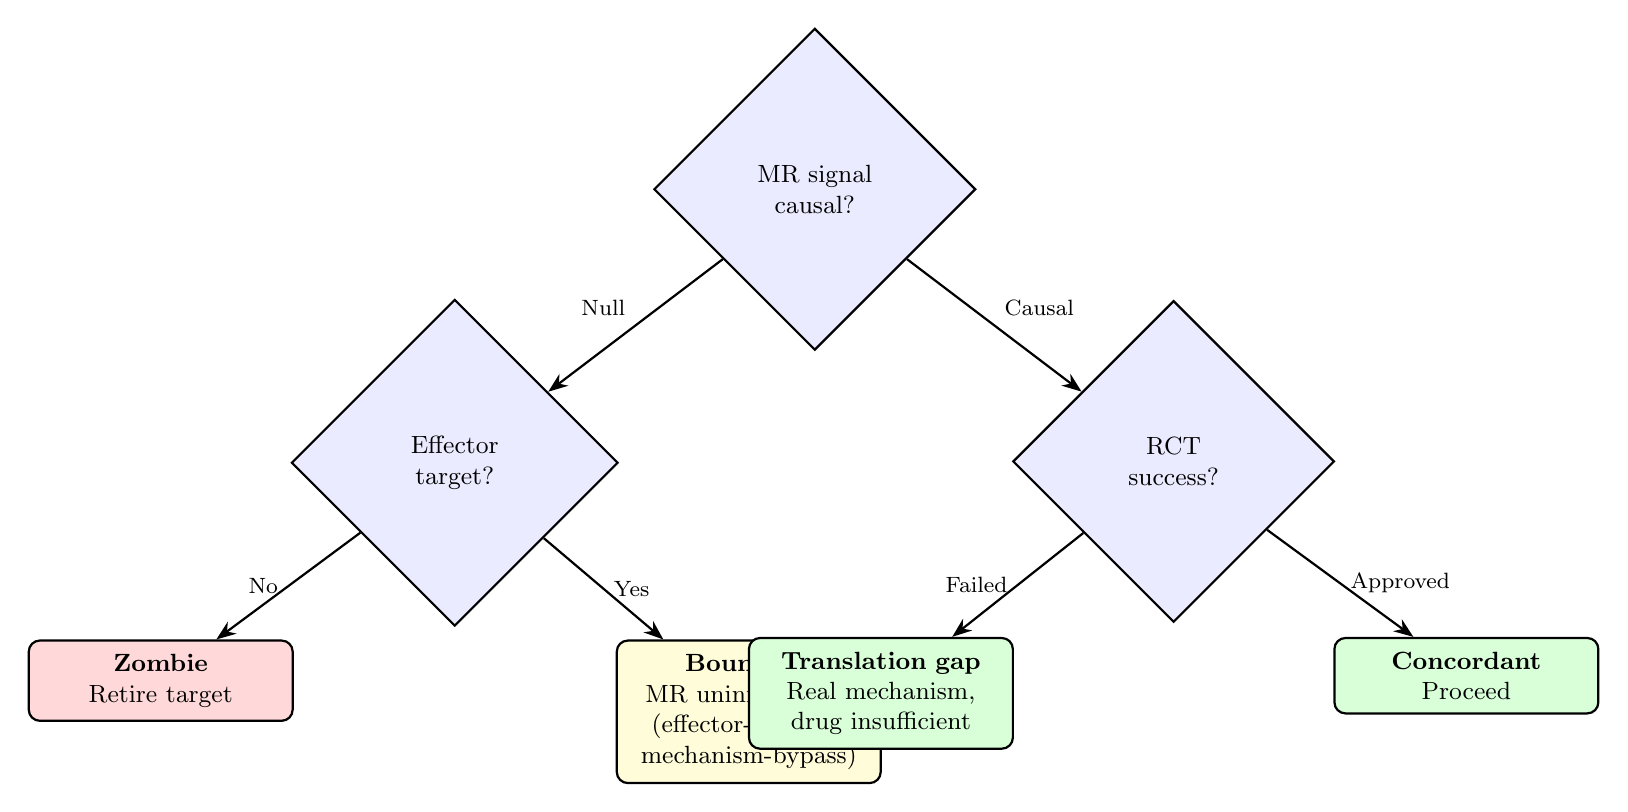
\begin{tikzpicture}[
    node distance=1.2cm and 2.0cm,
    decision/.style={diamond, draw, thick, fill=blue!8, text width=3.2cm, align=center, inner sep=2pt, font=\small},
    outcome/.style={rectangle, draw, thick, rounded corners, text width=3.0cm, align=center, inner sep=5pt, font=\small},
    good/.style={outcome, fill=green!15},
    bad/.style={outcome, fill=red!15},
    warn/.style={outcome, fill=yellow!15},
    arr/.style={-{Stealth[length=2.5mm]}, thick},
]
\node[decision] (mr) {MR signal\\causal?};
\node[decision, below left=1.4cm and 2.5cm of mr] (effector) {Effector\\target?};
\node[decision, below right=1.4cm and 2.5cm of mr] (rct) {RCT\\success?};
\node[bad, below left=1.2cm and 1.0cm of effector] (zombie) {\textbf{Zombie}\\Retire target};
\node[warn, below right=1.2cm and 1.0cm of effector] (bypass) {\textbf{Boundary}\\MR uninformative\\(effector-neutral.,\\mechanism-bypass)};
\node[good, below left=1.2cm and 1.0cm of rct] (translgap) {\textbf{Translation gap}\\Real mechanism,\\drug insufficient};
\node[good, below right=1.2cm and 1.0cm of rct] (success) {\textbf{Concordant}\\Proceed};

\draw[arr] (mr) -- node[above left, font=\footnotesize] {Null} (effector);
\draw[arr] (mr) -- node[above right, font=\footnotesize] {Causal} (rct);
\draw[arr] (effector) -- node[left, font=\footnotesize] {No} (zombie);
\draw[arr] (effector) -- node[right, font=\footnotesize] {Yes} (bypass);
\draw[arr] (rct) -- node[left, font=\footnotesize] {Failed} (translgap);
\draw[arr] (rct) -- node[right, font=\footnotesize] {Approved} (success);
\end{tikzpicture}
\caption{Screening decision tree for MR-based drug-target evaluation. A null MR signal indicates a zombie mechanism for risk-encoding targets, but is uninformative for effector-neutralization and mechanism-bypass targets. A causal MR signal is necessary but insufficient---translation-gap targets have real mechanisms but therapeutically insufficient drugs.}
\label{fig:screening}
\end{figure}

Despite growing evidence that genetic support predicts clinical success \cite{nelson2015,minikel2024}, we found no FDA or EMA guidance specifically addressing population-level genetic evidence (GWAS, MR) for target validation. Existing pharmacogenomics guidance concerns individual drug response---metabolism, dosing, adverse reactions---not the upstream question ``should we develop against this target?'' The closest touchpoints are the FDA Enrichment Strategies guidance (2019), endorsing genomic biomarkers for trial design, and the EMA's 2024 pharmacogenomics workshop, which acknowledged GWAS for understanding drug response variation. The boundary classes identified here---specifying where MR screening fails---could inform future regulatory frameworks for genetics-informed target selection. Whether boundary class membership also predicts post-market safety profiles (e.g., whether translation-gap drugs show different adverse-event patterns than zombie-targeting drugs that reached market through non-MR-supported pathways) is an open question with pharmacovigilance implications.

\subsection{Why etiologic concordance is necessary but insufficient}

The amyloid case illustrates a general principle. APOE4 is one of the strongest known genetic risk factors for any common disease (OR~3.46 per allele). Amyloid PET positivity robustly predicts AD conversion. The etiologic evidence is concordant. Drugs targeting amyloid clearance mostly fail.

The gap between etiologic concordance and interventional success reflects the difference between ``the mechanism is involved in pathogenesis'' and ``intervening on the mechanism at this stage reverses pathology.'' Amyloid accumulation may be an upstream causal factor in AD, but by the time clinical disease manifests, the downstream cascade (tau tangles, synaptic loss, neuroinflammation) may have become self-sustaining---though this mechanistic explanation remains a hypothesis rather than an established fact. The recent FDA approvals of lecanemab and donanemab via accelerated and traditional pathways remain controversial, with debate over whether statistically significant slowing on CDR-SB (27--35\%) constitutes clinical benefit. An estimated \$40 billion in failed trials \cite{cummings_zhong2014} targeted a mechanism that was etiologically valid but therapeutically insufficient.

The method performs more cleanly on MS than on AD. MS mechanism families map to specific biological pathways (B-cell depletion, vitamin~D, EBV) with relatively homogeneous drug targets within each family. AD families are more heterogeneous: ``amyloid'' encompasses production-pathway inhibitors, passive immunotherapy, and active immunotherapy, which may have distinct mechanisms of failure.

\subsection{Limitations}
\label{sec:limitations}

The etiologic-only analysis classifies 8 of 38 holdout drugs---the remainder fall in families without multi-type etiologic evidence. The analysis is powered to demonstrate proof-of-concept (7/8 correct), not to establish population-level accuracy. The retrospective analysis including RCT evidence is circular for families whose RCT arm derives from holdout drugs---it should be interpreted as concordance, not prediction.

\paragraph{Threshold sensitivity and mixed contrasts.} The threshold $d = 0.10$ was chosen on substantive grounds (Cohen's negligible-effect boundary), not optimized. MR effect sizes enter on their native contrast (per-SD, per-unit, per-allele, per-genotype), and the Chinn $d$ inherits that contrast. Of 32 scored families, 15 use per-SD MR effects, 7 use per-allele, 5 use per-unit, 1 per-genotype, and 3 have null signals where contrast is irrelevant (pre-registered scale analysis, SHA \texttt{4b0a652}). Universal rescaling to a common per-SD basis is infeasible: the conversion factors (SD of exposure per allele or per unit) are unavailable for most non-per-SD families. Only IL-6R is explicitly rescaled in this paper. The $d = 0.10$ threshold is therefore applied across incomparable scales---a pragmatic choice, since no universal rescaling exists.

Anti-CD20-MS is threshold-sensitive and contrast-dependent: its MR $d = 0.103$ (per-SD circulating FCRL3 protein) clears by 0.003. At $d = 0.099$ the classification flips to discordance, misclassifying four approved drugs. At thresholds of $d = 0.08$ and $d = 0.12$, all other neuro/cardio classifications are unchanged (7/8 and 7/7 correct at both). Three additional families are threshold-sensitive at narrower ranges: IL-6R ($d = 0.083$) and CTLA-4-RA ($d = 0.083$) would flip from null to causal at a lower threshold; Uric acid ($d = 0.037$) is robustly null. The overall result is robust to perturbation but three individual classifications depend on the exact threshold.

\paragraph{Autoimmune OBS construct.} The autoimmune domain uses case-control SMDs rather than epidemiological ORs as the OBS measure. Three families (CTLA-4-RA, JAK-STAT-RA, CD20-RA) have author-estimated SMDs ($d = 0.50$) rather than meta-analysis-sourced values. All three are well above the $d = 0.10$ threshold, so their classification is insensitive to the estimate; moreover, since the invariance result shows OBS carries zero discriminative information, these values cannot affect any classification even in principle. The identical round values should be understood as nominal placeholders indicating ``clearly non-trivial,'' not precise measurements. Autoimmune accuracy is reported separately from neuro and cardio and the domains are never pooled.

\paragraph{Family granularity.} Mechanism families are defined at the biological-pathway level, but the granularity is not uniquely determined. Semaglutide (assigned to Metabolic-AD) is a GLP-1 agonist with both metabolic and direct neuroprotective effects; the family assignment assumes the metabolic pathway is the relevant one. In the cardiometabolic domain, ``HDL/CETP'' could be split into genetic HDL-raising (null for CHD) and pharmacological CETP inhibition (which also raises LDL and has off-target toxicity). The family definitions are a degree of freedom, and different choices could change classifications.

\paragraph{Instrument-target alignment.} MR instruments are proxies for drug mechanisms, not direct models. The FCRL3 instrument for Anti-CD20-MS captures circulating FCRL3-mediated B-cell biology but not the ADCC mechanism of ocrelizumab; the IL6R instrument for IL-6 pathway inhibition targets the receptor while ziltivekimab targets the ligand. These mismatches do not invalidate the etiologic signal (both concern the same biological pathway) but they weaken the correspondence between MR evidence and drug mechanism.

\paragraph{Estimand alignment.} The concordance rule compares effect sizes targeting different causal estimands: observational ORs conditional on measured confounders, MR estimates approximating lifelong exposure modification, and RCT estimates capturing a specific intervention over a defined period \cite{hernan2016}. The Chinn $d$ standardizes scale, not estimand. For zombie mechanisms, the mismatch is immaterial---a null MR signal indicates no causal pathway regardless of the observational estimand. For concordant mechanisms, agreement in sign and magnitude is suggestive rather than confirmatory, and translation-gap failures could partly reflect estimand differences rather than biological insufficiency.

\paragraph{Ascertainment.} Mechanism families were selected from well-known programs, introducing possible outcome-influenced selection. The prospective predictions (Lp(a), IL-6) and pre-registered extensions mitigate this concern. Prospective validation at trial readout is the definitive test.

\paragraph{Family-level vs.\ drug-level accuracy.} The 24/32 (75\%) accuracy is computed at the mechanism-family level. Families contain different numbers of drugs: Anti-CD20-MS maps to four approved drugs; Amyloid-AD maps to fourteen (twelve failed, two approved). A misclassified family with many drugs produces more incorrect drug-level predictions than one with a single drug. In neuroepidemiology, where drug-level mapping was performed, 8 drugs mapped to 4 classified families (7/8 correct), and 14 mapped to Amyloid-AD (classified as translation-gap in Stage~2). For extension domains, only family-level accuracy is reported because exhaustive drug-to-family mapping was not performed. Family-level accuracy is the appropriate unit for evaluating the diagnostic taxonomy---the taxonomy classifies mechanisms, not individual compounds---but drug-level accuracy would better quantify the practical screening value of MR-null status.

\paragraph{Extension provenance.} The extension families were added in two blind amendments, each pre-registered before effect sizes were retrieved (Amendment~1 commit \texttt{1f300a9}; Amendment~2 commit \texttt{12ea0ed}). The author (ET) selected extension families with access to the framework rules and existing domain coverage, but without access to classifier code, accuracy statistics, or prior classification results. Every declared family was scored regardless of outcome; none were dropped post hoc. The extension accuracy (6/10, 60\%) does not reach statistical significance in isolation (one-sided binomial $p = 0.17$ against chance) and should be interpreted as a replication exercise mapping boundary conditions, not as a standalone confirmatory result.

\section{Conclusions}

The MR-only and cross-design rules produce identical classifications across all 32 scored families---an invariance that holds at every threshold tested ($d = 0.05$ to $0.20$) and reflects a selection effect: mechanisms reaching Phase~III have non-trivial observational support by construction. The predictive work reduces to MR-null status. The cross-design framework's contribution is diagnostic: it separates the eight misclassified families into two structurally distinct groups that MR alone cannot distinguish.

Five families have null MR signals yet succeed clinically (effector-neutralization and mechanism-bypass). Three families have causal MR signals yet fail clinically (translation gaps and exposure mismatches). This two-way partition falls directly from the MR $d$ axis and requires no additional parameters. The finer five-class taxonomy---effector-neutralization, small-effect, translation-gap, exposure-mismatch, and mechanism-bypass---offers mechanistic hypotheses for each type of miss. These labels are proposals on $n = 8$, grounded in pharmacological reasoning but requiring prospective replication (Table~\ref{tab:provenance}).

A null MR signal is a strong negative indicator---the mechanism is likely a zombie. A positive MR signal is necessary but insufficient: developers should ask whether the target is a disease effector, whether the drug recapitulates the instrumented exposure, and whether the pharmacological perturbation exceeds the scale of genetic variation. Answering these questions requires the diagnostic framework; the MR screen alone cannot.

\section*{Abbreviations}
AD: Alzheimer's disease;
ADCC: Antibody-dependent cellular cytotoxicity;
AMD: Age-related macular degeneration;
BACE: Beta-site amyloid precursor protein cleaving enzyme;
BC: Breast cancer;
BMI: Body mass index;
CDR-SB: Clinical Dementia Rating Sum of Boxes;
CETP: Cholesteryl ester transfer protein;
CFH: Complement factor H;
CI: Confidence interval;
COPD: Chronic obstructive pulmonary disease;
CRC: Colorectal cancer;
CRP: C-reactive protein;
CVD: Cardiovascular disease;
EBV: Epstein-Barr virus;
eQTL: Expression quantitative trait locus;
ER: Estrogen receptor;
FCRL3: Fc receptor-like 3;
GA: Geographic atrophy;
GEN: Genetic/causal evidence;
GLP-1R: Glucagon-like peptide-1 receptor;
GRADE: Grading of Recommendations, Assessment, Development and Evaluations;
GWAS: Genome-wide association study;
HDL: High-density lipoprotein;
HF: Heart failure;
HR: Hazard ratio;
HRT: Hormone replacement therapy;
IGF-1: Insulin-like growth factor 1;
IL: Interleukin;
LDL: Low-density lipoprotein;
MDD: Major depressive disorder;
MR: Mendelian randomization;
MS: Multiple sclerosis;
OBS: Observational evidence;
OR: Odds ratio;
PCSK9: Proprotein convertase subtilisin/kexin type 9;
PET: Positron emission tomography;
pQTL: Protein quantitative trait locus;
RA: Rheumatoid arthritis;
RCT: Randomized controlled trial;
RR: Relative risk;
SBP: Systolic blood pressure;
SD: Standard deviation;
SGLT2: Sodium-glucose co-transporter 2;
SLC6A4: Solute carrier family 6 member 4 (serotonin transporter);
SOST: Sclerostin gene;
SSRI: Selective serotonin reuptake inhibitor;
SMD: Standardized mean difference;
T2D: Type 2 diabetes;
TG: Triglycerides;
TNF: Tumor necrosis factor;
TSLP: Thymic stromal lymphopoietin;
WHIMS: Women's Health Initiative Memory Study;
5-HTTLPR: 5-HT transporter-linked polymorphic region.

\subsection*{Data Availability Statement}
All effect sizes were extracted from published studies cited in the manuscript. The deterministic classifier (\texttt{classify\_families.py}), robustness analysis code (\texttt{robustness\_analyses.py}), and the complete classification dataset (41 families with effect sizes, CIs, and sources) are available at \url{https://github.com/elliottower/cross-design-evidence-discordance} (commit \texttt{bf7f175}) with a permanent archive at Zenodo (DOI: \url{https://doi.org/10.5281/zenodo.21227354}). Pre-registration commits with SHAs are documented in the repository. No novel datasets were generated.

\subsection*{Ethics Statement}
This study analyzed published, aggregate-level effect sizes from existing meta-analyses and Mendelian randomization studies. No individual-level patient data were accessed. Ethical approval was not required in accordance with institutional and national guidelines.

\subsection*{Author Contributions}
ET conceived the study, assembled the evidence catalog, designed and implemented the classification rule, performed all analyses, and wrote the manuscript. The author read and approved the final manuscript.

\subsection*{Funding}
This research received no specific grant from any funding agency in the public, commercial, or not-for-profit sectors.

\subsection*{Acknowledgements}
Not applicable.

\subsection*{Conflict of Interest Statement}
The author declares no competing interests.

\subsection*{Use of AI-Assisted Technologies}
Claude (Anthropic) was used as a writing and analysis assistant during manuscript preparation. The author directed all analytical decisions, verified all numerical results against source data, and takes full responsibility for the content. The classification rule, effect-size data, and all reported results were independently validated by the author. No AI tool is listed as an author.

\bibliographystyle{unsrtnat}
\bibliography{references}

\end{document}
